\clearpage
%%=========================================
\section{Surface Analysis of As-Received Substrate B}\label{sec:subBa}
% Substrate B
In previous work \citep{lauten2017characterisation}, the as-received (111)B-oriented substrate B was characterised for polishing damage, defects, and residual particles using optical microscopy and \ac{sem} with \ac{eds}. The results are reiterated in this section to better present the full scope of the study. In addition to the previously used methods, \ac{afm}, near-\ac{ir} transmission microscopy, and \ac{ftir} were used to study the as-received substrate.

Fig.~\ref{fig:subBa_om_df} shows typical dark field images from the surface of substrate B at the corner, edge, and centre of the substrate. Polishing scratches in all directions and with varying width can be observed, both at the centre and towards the edges, on the surface of substrate B. Big particles and morphological defects with a diameter between \SI{10}{\micro\metre} and \SI{50}{\micro\metre}, as well as smaller particles and morphological defects with diameter \SI{<10}{\micro\metre}, are present on the surface. By counting the number of spots in the dark field image, the particle and morphological defect density is estimated to be \SI{1e5}{\centi\metre^{-2}}, both at the centre and at the edges of the surface of substrate B. Also, here the particle and morphological defect density refers to the sum of all light scattering objects \SI{>0.5}{\micro\metre} in size.
% --- Measured with tolerance of 10 using ImageJ. One pixel are 2250/2048 um.
%       Centre: 5739 partikler på 2048x1536 --> 151151 particles per cm^2
%       Edges: 3927 partikler på 1877x1522 --> 113888 particles per cm^2
%       Corner: 5327 partikler på 1848x1486 --> 158000 particles per cm^2

\begin{figure}[htbp]
    \centering
    \mySubfigure{\linewidth}{LM_DF_C389523A_M005_centre.jpg}[fig:subBa_om_df_centre]
    \par\bigskip
    \mySubfigure{0.49\linewidth}{LM_DF_C389523A_M005_centreEdge.jpg}[fig:subBa_om_df_edge]
    \hfill
    \mySubfigure{0.49\linewidth}{LM_DF_C389523A_M005_corner.jpg}[fig:subBa_om_df_corner]
    \caption[Dark field images of substrate B.]{Dark field images of substrate B captured through the optical microscope Leica DM RXA2 at the \subref{fig:subBa_om_df_centre} centre; \subref{fig:subBa_om_df_edge} edge; and \subref{fig:subBa_om_df_corner} corner of the substrate.}
    \label{fig:subBa_om_df}
\end{figure}

The difference between substrate A and substrate B is significant. Substrate B has a density of particles and morphological defects that is 100-1000 times larger than the density of particles and morphological defects on the surface of substrate A. This can be explained by the more thorough preparation that substrate A has been subjected to. Substrate A has had a final polishing and an etch before being delivered, while substrate B is roughly polished and particles on the surface have not been removed.

A comparison between the dark field image and a \ac{sem} image of the same area of substrate B, as seen in Fig.~\ref{fig:LM_SEM_C3895}, reveal that the brightest spots in the dark field image are from cavities in the substrate surface and that particles as small as \SI{0.5}{\micro\metre} can be seen in the dark field image. The dark stains on the other hand are not visible in the dark field image.

\begin{figure}[htbp]
    \centering
    %\mySubfigure[Dark field optical microscope image.]{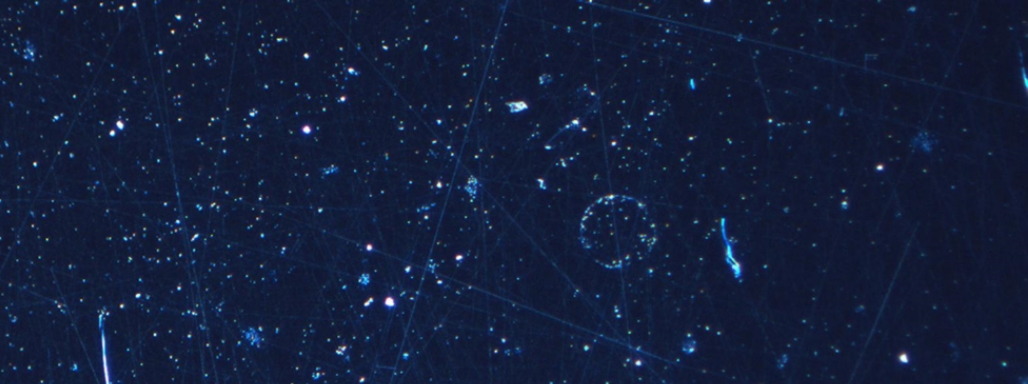
\includegraphics[width=1\linewidth]{C-3895-23A_centre_LM.jpg}\label{fig:C-3895-23A_centre_LM}}
    %\mySubfigure[SEM image at a magnification of 60$\times$.]{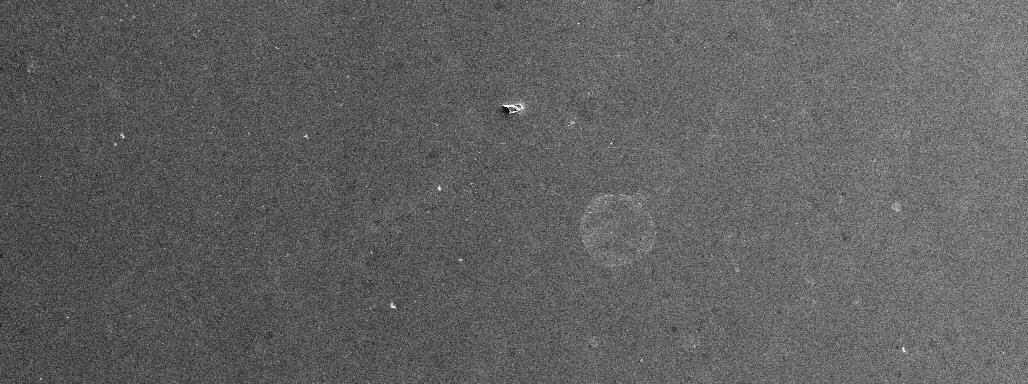
\includegraphics[width=1\linewidth]{C-3895-23A_centre_SEM.jpg}\label{fig:C-3895-23A_centre_SEM}}
    \mySubfigure{0.36\linewidth}{C-3895-23A_edge_LM_500_overview.jpg}[fig:C-3895-23A_edge_LM_500_overview]
    \hfill
    \mySubfigure{0.60\linewidth}{C-3895-23A_edge_SEM_500_overview.jpg}[fig:C-3895-23A_edge_SEM_500_overview]
    \caption[Comparison of dark field microscopy and \ac{sem} images.]{Comparison of \subref{fig:C-3895-23A_edge_LM_500_overview} a dark field microscopy image captured through the optical microscope Leica DM RXA2 and \subref{fig:C-3895-23A_edge_SEM_500_overview} \iacf{sem} image taken at the same location on the as-received substrate B as the dark field image.}
    \label{fig:LM_SEM_C3895}
\end{figure}

A \ac{sem} image mapping of substrate B was done at points in a grid of $11\times11$ grid points. The distance between neighbouring points was \SI{2.60}{\milli\metre} and the distance from the edge to the outer points was \SI{2.00}{\milli\metre}. A low magnification \ac{sem} image (60$\times$) and a higher magnification image (500$\times$) were acquired at every grid point. This mapping will be used in future studies of substrate B when correlation between defect density and preparation methods is going to be measured.

%A particle and morphological defect density of features \SI{>0.5}{\micro\metre} of \SI{1e5}{\centi\metre^{-2}} at both the centre and at the edges of the substrate was observed. Substrate B had polishing scratches that were between 10 and \SI{100}{\nano\metre} wide. A large amount of voids with sizes ranging from \SI{5}{} to \SI{100}{\micro\metre} were observed on the surface of substrate B. 

%Most of the particles \SI{>1}{\micro\metre} on the surface of substrate B were \ce{CdZnTe} particles with lengths of between \SI{50}{} and \SI{100}{\micro\metre} that could be debris from the cutting of the substrate, but some carbon based particles was also observed with lengths of \SI{25}{\micro\metre}. Most of the particles \SI{<1}{\micro\metre} on the surface of substrate B were residual \ce{Al2O3} and \ce{SiO2} polishing grit with diameter of between \SI{50}{} and \SI{100}{\nano\metre}.  In addition, iron particles, which could be possible remainders of polishing slurry, and particles containing \ce{Na} and \ce{Cl}, which could be possible remainders of polishing slurry cleaner, were observed on the surface of substrate B.

%%=========================================
%\section{Particles and Defects on Substrate B}


One of the \ac{sem} images from the grid at the middle of substrate B taken at low magnification (60$\times$), see Fig.~\ref{fig:C-3895-23A_F08_x060}, shows some bright stains at the top of the image, a dark spot down in the right corner, and a lot of bright spots all over. The \ac{sem} image of the same area at higher magnification (500$\times$), see Fig.~\ref{fig:C-3895-23A_F08_x500}, reveals that there are surface scratches, dark stains of different sizes and some even smaller bright spots on the surface. These features need to be studied at even higher magnifications to be able to identify what they are.\todo{And?}

\begin{figure}[htbp]
    \centering
    \mySubfigure{0.49\linewidth}{C-3895-23A_F08_x060.jpg}[fig:C-3895-23A_F08_x060]
    \hfill
    \mySubfigure{0.49\linewidth}{C-3895-23A_F08_x500.jpg}[fig:C-3895-23A_F08_x500]
    \caption[\Ac{sem} images of a typical area in the middle of substrate B.]{\Acf{sem} images of a typical area in the middle of substrate B at \subref{fig:C-3895-23A_F08_x060} $60\times$ magnification; and \subref{fig:C-3895-23A_F08_x500} $500\times$ magnification.}
    \label{fig:SEM_C389523_overview}
\end{figure}

\subsection{Particles and Surface Features}
Seven different types of particles and surface features were observed on the surface of substrate B, see Fig.~\ref{fig:subBa_sem_w_eds}. They will be described and identified in the following.
%\mySubfigure[SEM.]{0.44\linewidth}{C-3895-23_09_m001.jpg}
    %\mySubfigure[SEM.]{0.44\linewidth}{C-3895-23A_edx7_m002.jpg}
    %\mySubfigure[SEM.]{0.44\linewidth}{C-3895-23A_edx7_m003.jpg}
\begin{figure}[htbp]
    \centering
    \begin{subfigure}[t]{\textwidth}
          \begin{minipage}[t]{0.48\linewidth}
            \centering
            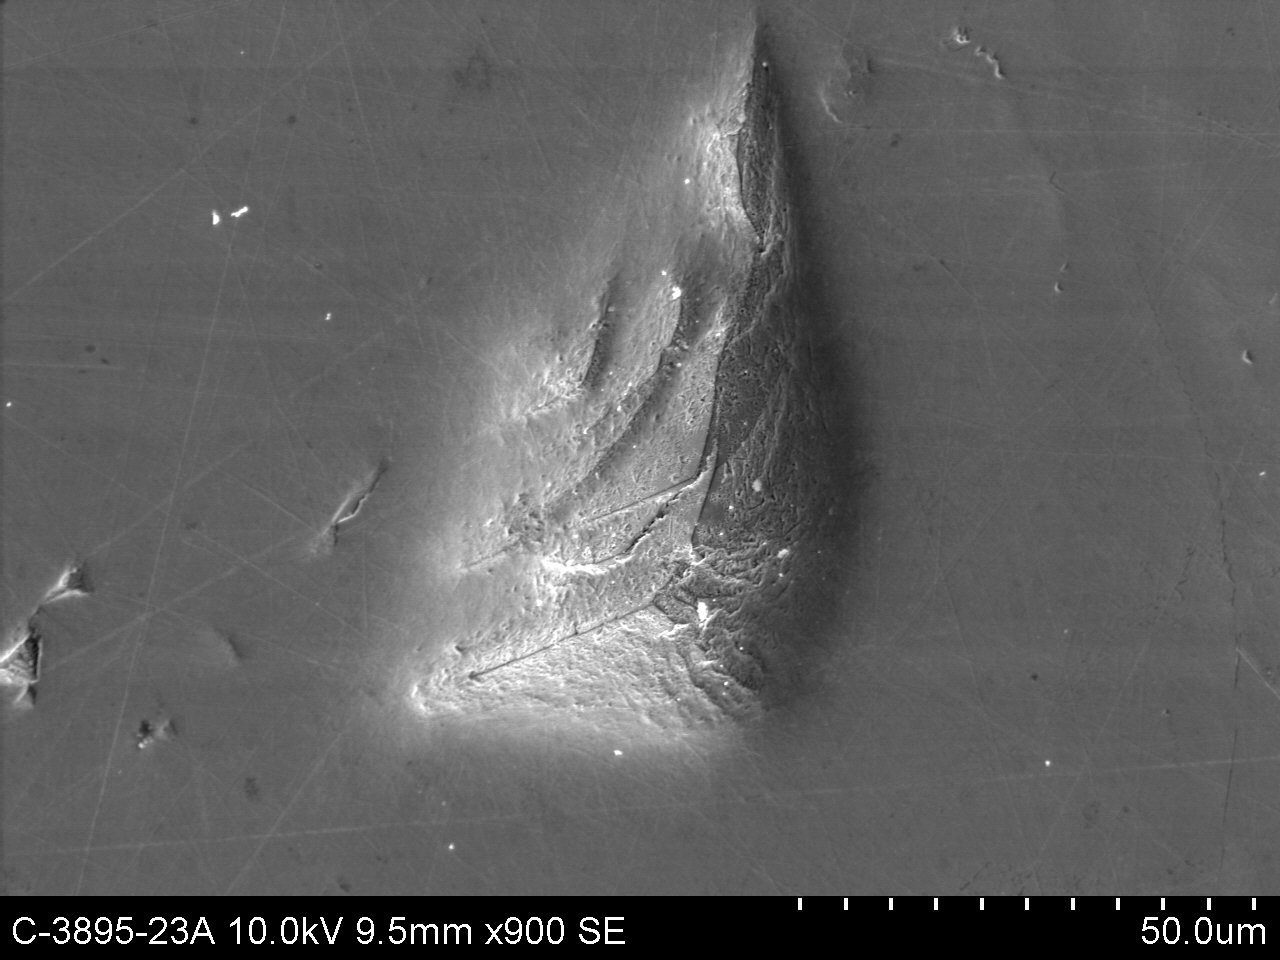
\includegraphics[width=\linewidth]{C-3895-23_09_m001.jpg}%C-3895-23A_edx3_m001.jpg}
          \end{minipage}
          \hfill
          \begin{minipage}[t]{0.48\linewidth}
            \centering
            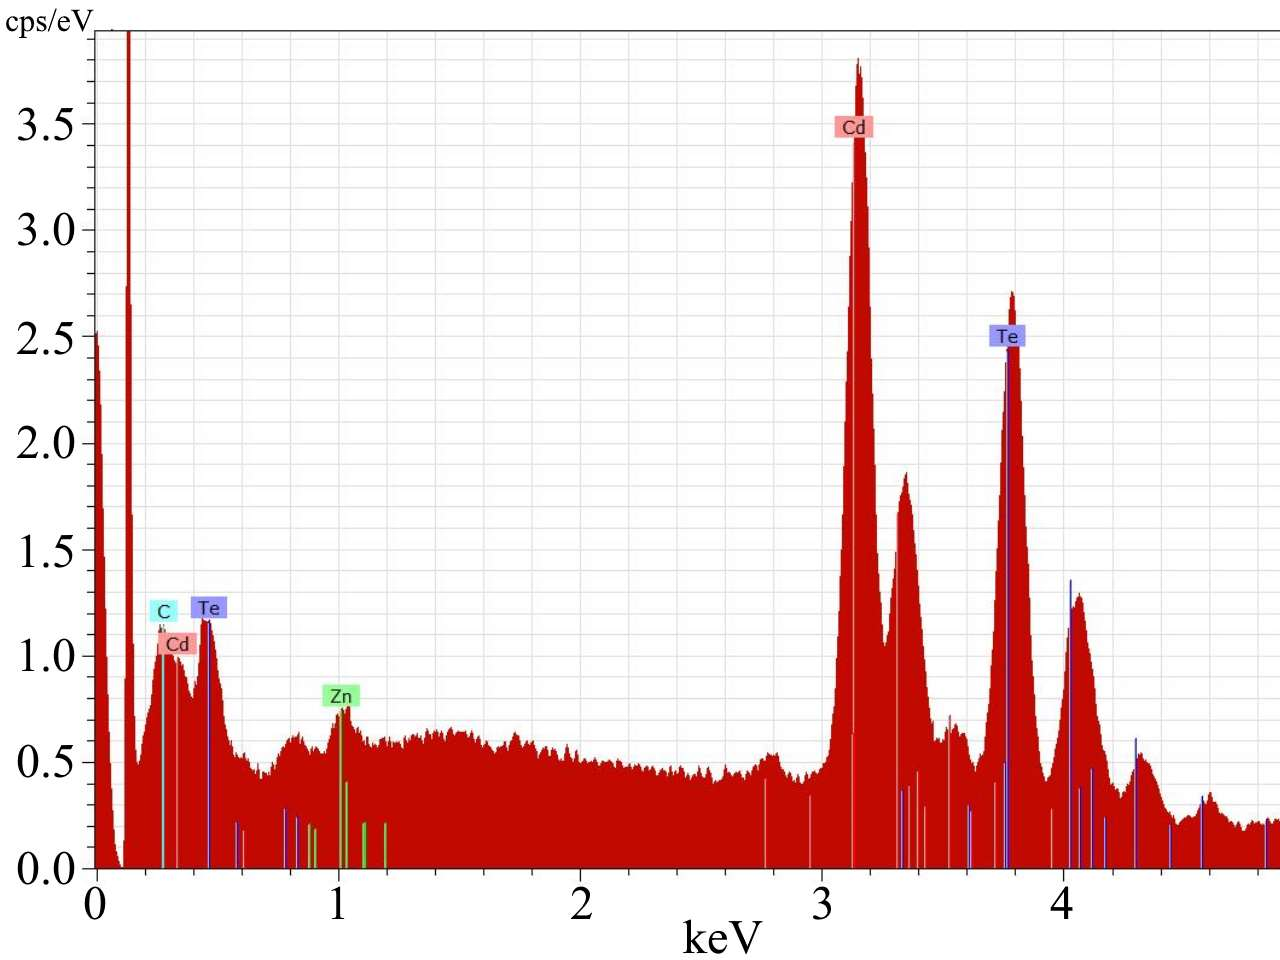
\includegraphics[width=\linewidth]{C-3895-23A_edx3_m001_eds.jpg}
          \end{minipage}
        \caption{\ac{sem} image of a void in the substrate surface at a magnification of 15000$\times$. The corresponding \ac{eds} spectrum reveals that the void consists of the same material as the substrate, \ce{Cd_{0.96}Zn_{0.04}Te}.}\label{fig:SEM_C389523_void_eds}
    \end{subfigure}%
    \par\bigskip
    \begin{subfigure}[t]{\textwidth}
          \begin{minipage}[t]{0.48\linewidth}
            \centering
            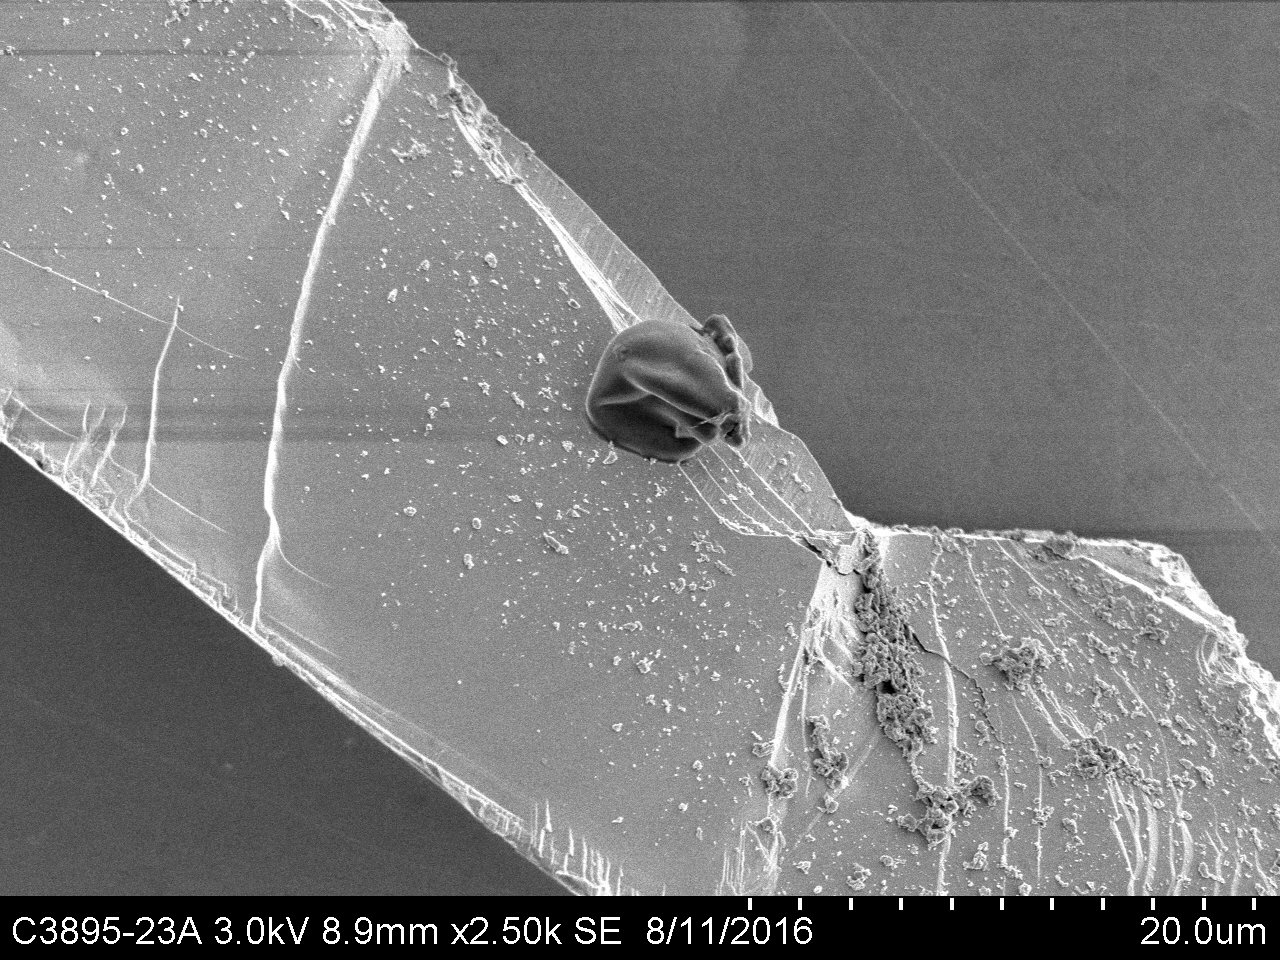
\includegraphics[width=\linewidth]{C-3895-23Af2_m002.jpg}
          \end{minipage}
          \hfill
          \begin{minipage}[t]{0.49\linewidth}
            \centering
            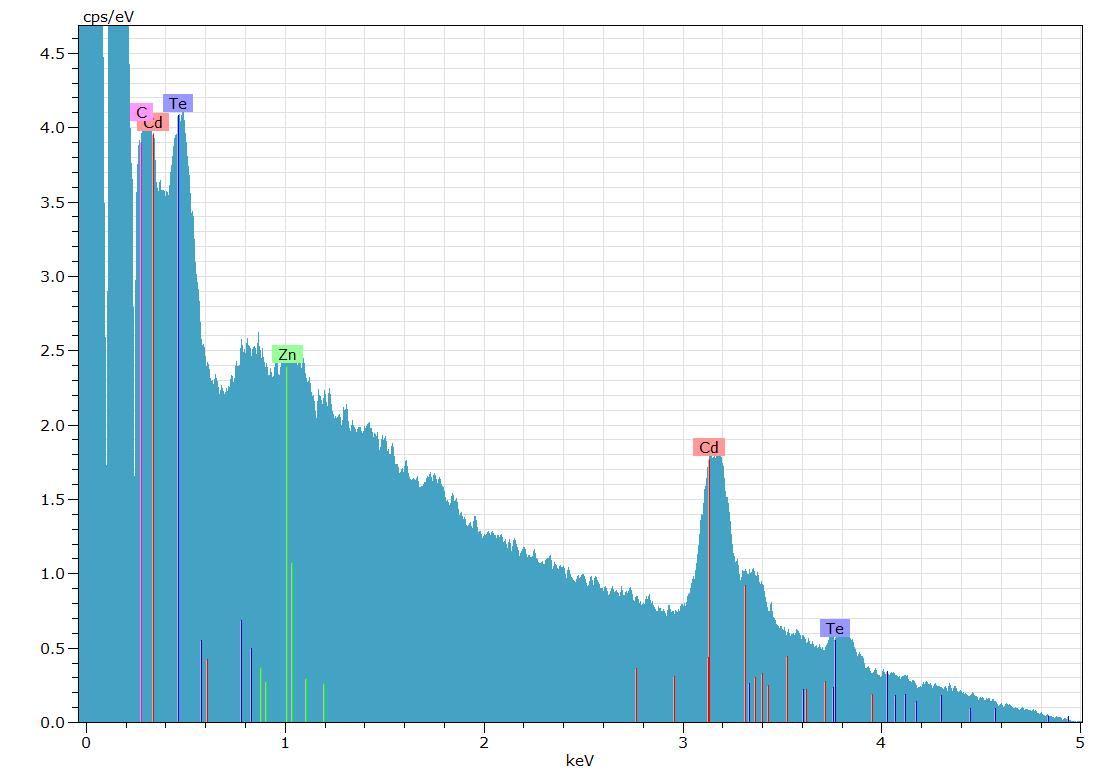
\includegraphics[width=\linewidth]{CdZnTe_eds.jpg}
          \end{minipage}
          %\begin{minipage}[t]{0.49\linewidth}
          %  \centering
          %  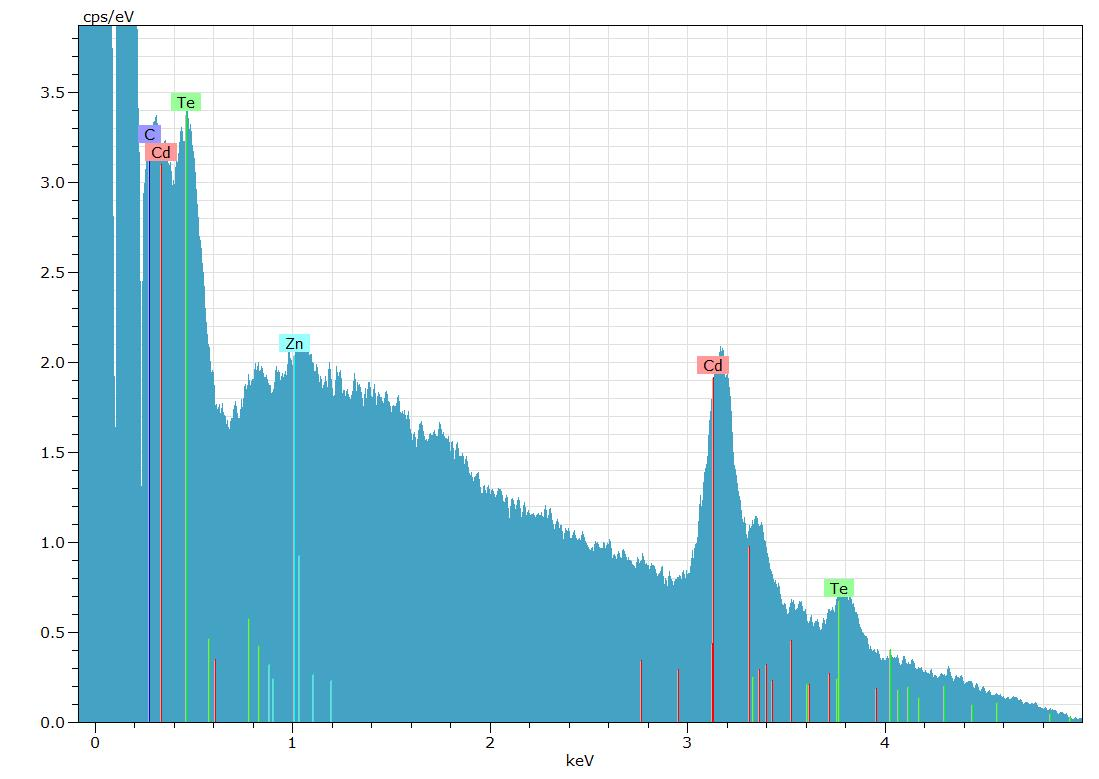
\includegraphics[width=\linewidth]{CdZnTe_eds_substrate.jpg}
          %\end{minipage}
        \caption{\Ac{sem} image of a \ac{czt} particle at a magnification of $2500\times$ and the corresponding \ac{eds} spectrum. The spectrum reveals that the particle consists of the same material as the substrate, \ce{Cd_{0.96}Zn_{0.04}Te}.}\label{fig:SEM_B_particulates_eds}
    \end{subfigure}%
    \par\bigskip
    \begin{subfigure}[t]{\textwidth}
          \begin{minipage}[t]{0.49\linewidth}
            \centering
            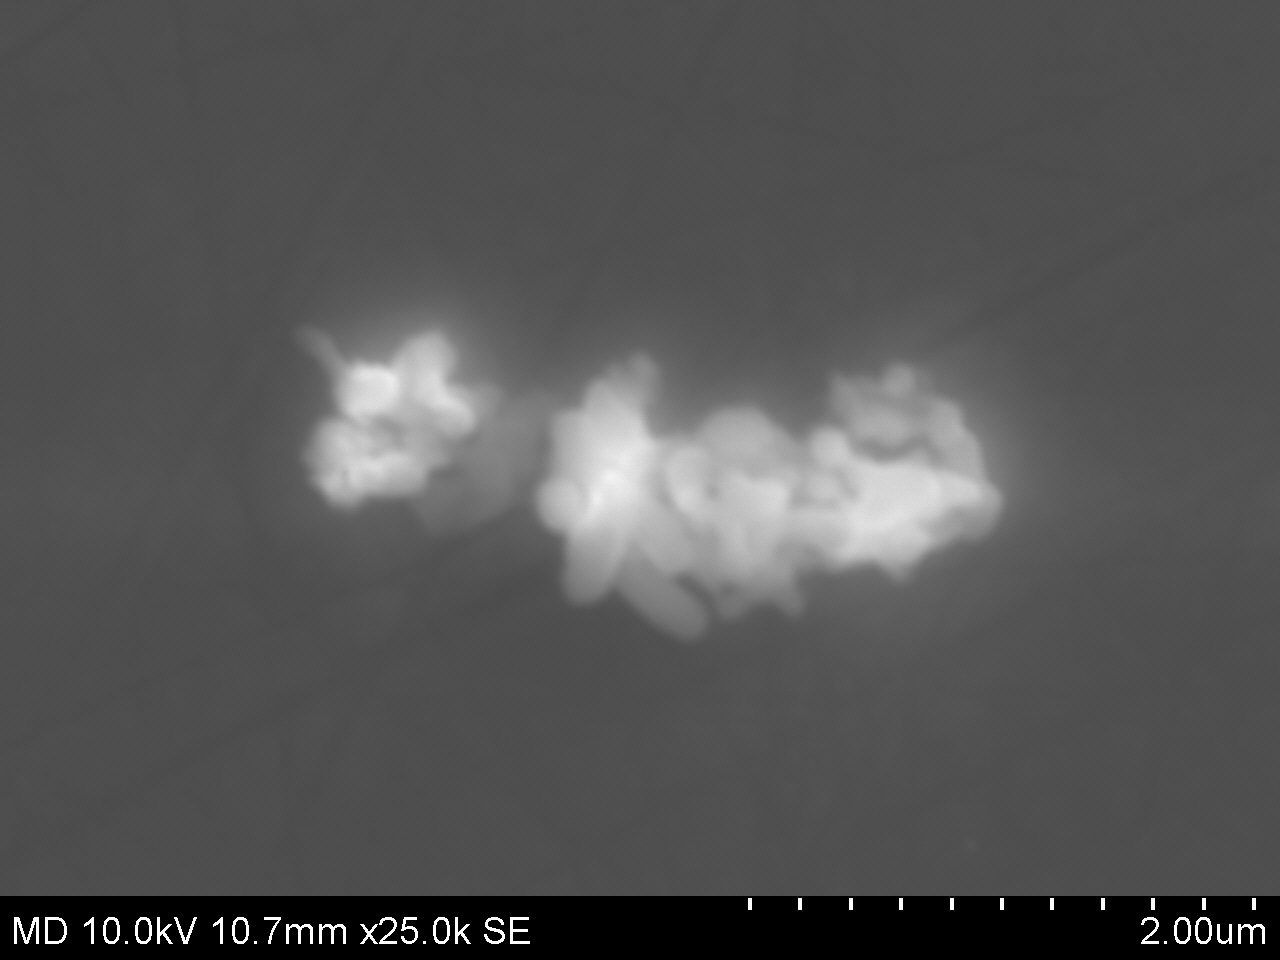
\includegraphics[width=\linewidth]{alumina02_sem.jpg}
          \end{minipage}
          \hfill
          \begin{minipage}[t]{0.49\linewidth}
            \centering
            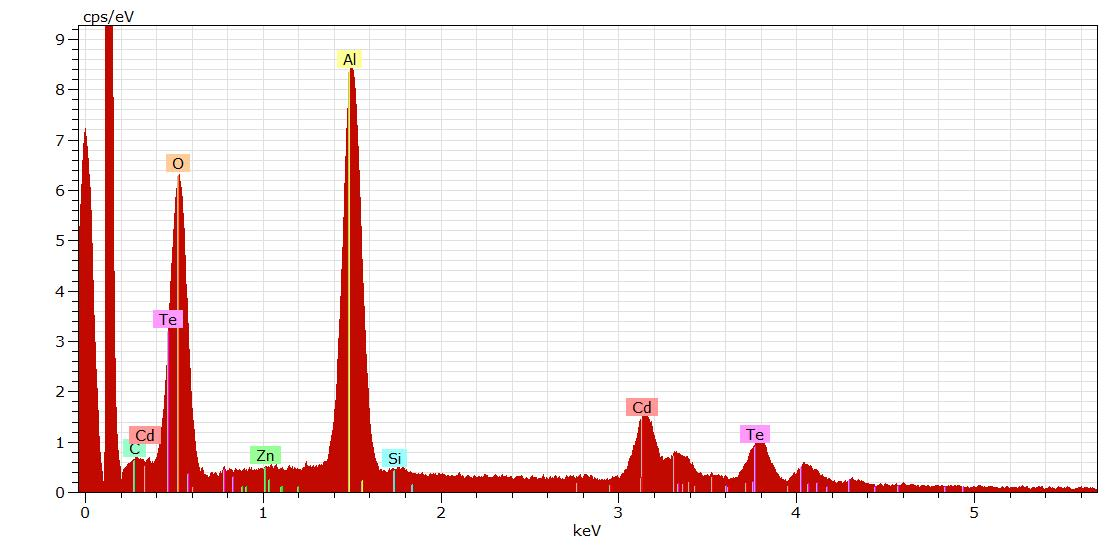
\includegraphics[width=\linewidth]{alumina02_eds.jpg}
          \end{minipage}
        \caption{\Ac{sem} image of an agglomeration of alumina (\ce{Al2O3}) polishing grit at a magnification of 25000$\times$ and the corresponding \acf{eds} spectrum.}\label{fig:subBa_polishing-grit_alumina}
    \end{subfigure}%
    \caption[\Ac{sem} images and \ac{eds} spectra of particles found on as-received substrate B.]{High resolution \acf{sem} images of particles found on the as-received substrate B and the corresponding \ac{eds} spectra of the particles.}\label{fig:subBa_sem_w_eds}
\end{figure}
%
\begin{figure}[htbp]
\ContinuedFloat
    \centering
    \begin{subfigure}[t]{\textwidth}
          \begin{minipage}[t]{0.49\linewidth}
            \centering
            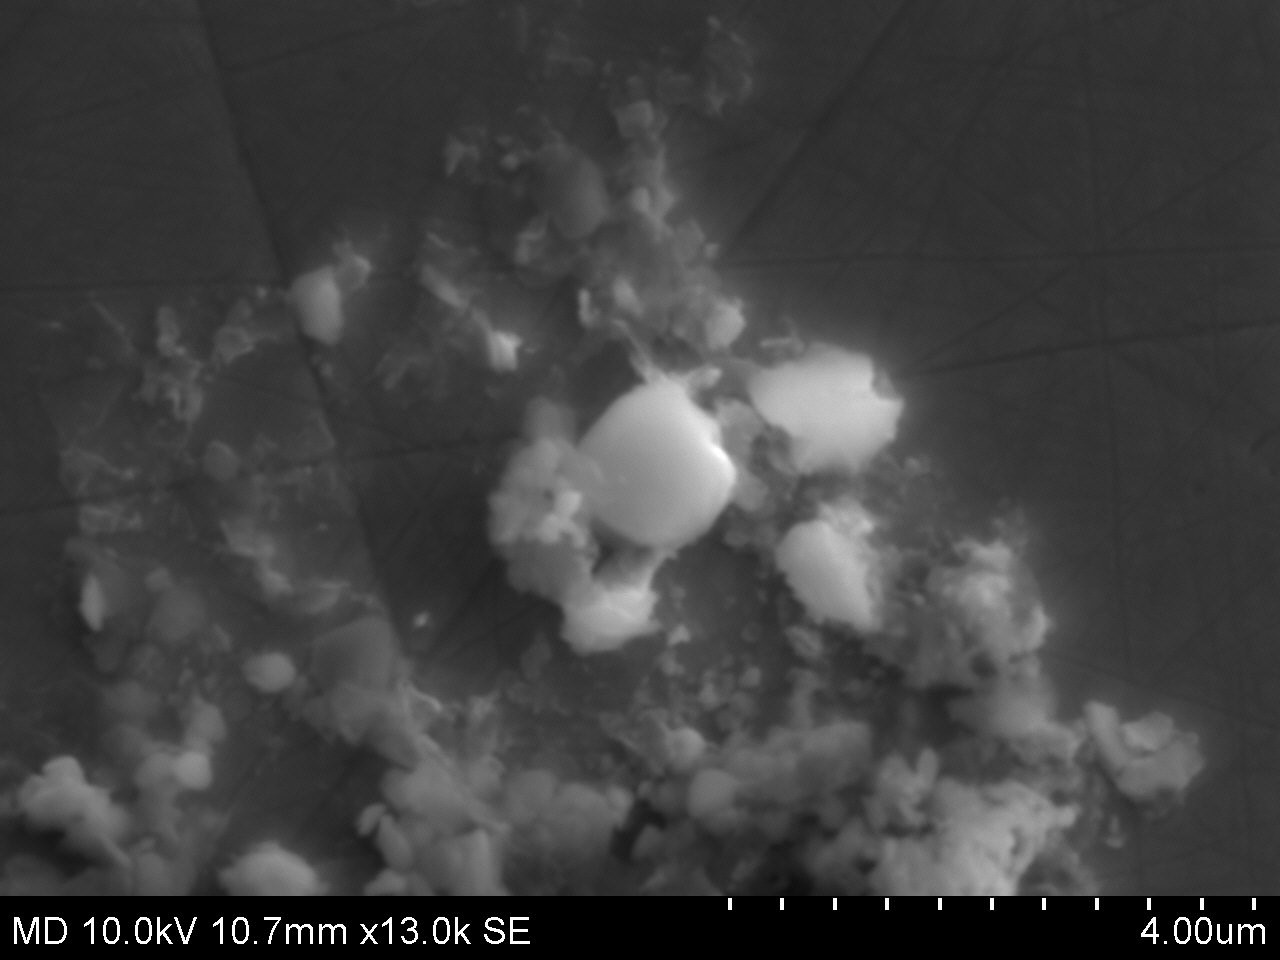
\includegraphics[width=\linewidth]{subB_silica_sem.jpg}
          \end{minipage}
          \hfill
          \begin{minipage}[t]{0.49\linewidth}
            \centering
            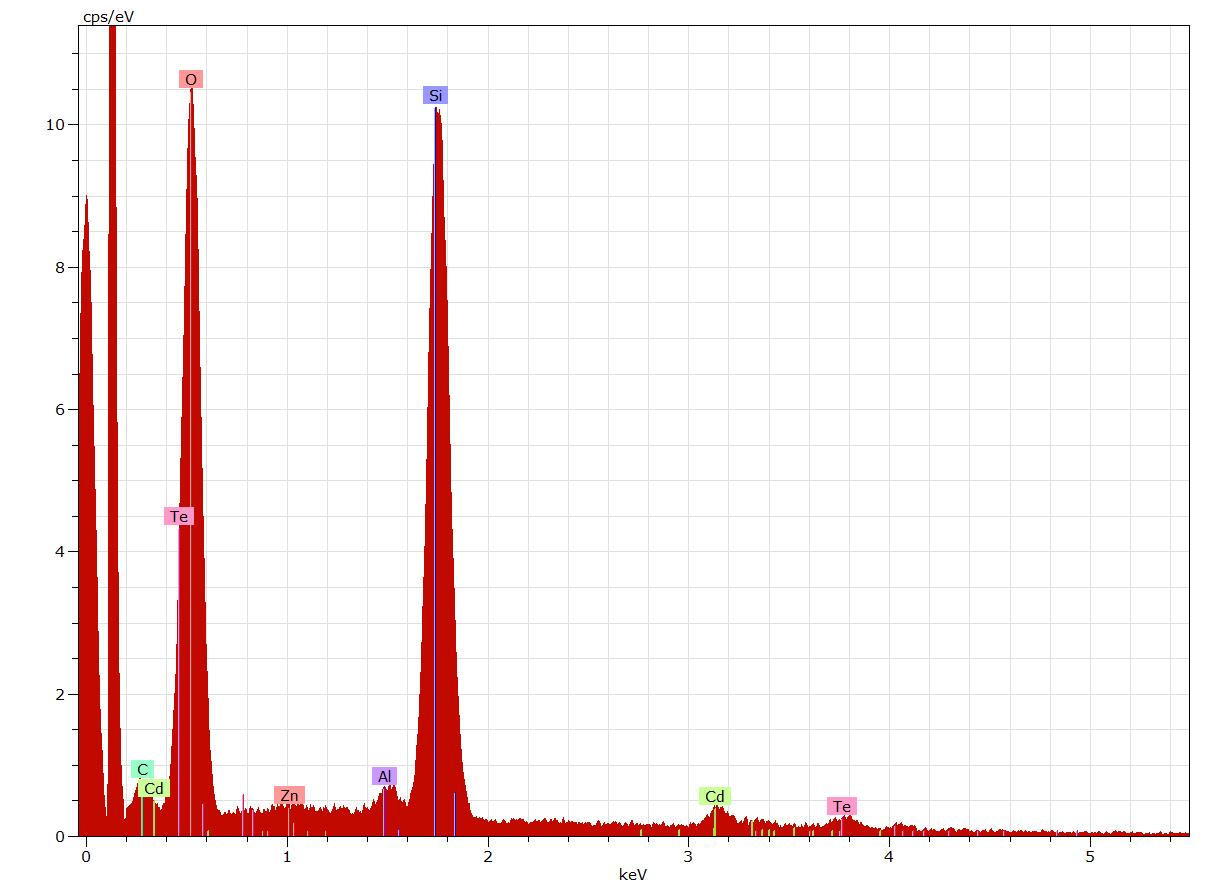
\includegraphics[width=\linewidth]{subB_silica_eds.jpg}
          \end{minipage}
        \caption{\Ac{sem} image of particles on substrate B at a magnification of $13000\times$ and the corresponding \ac{eds} spectrum of the largest piece. The spectrum reveals that the particle consists of silica (\ce{SiO2}).}\label{fig:subBa_polishing-grit_silica}
    \end{subfigure}%
    \par\bigskip
    \begin{subfigure}[t]{\textwidth}
          \begin{minipage}[t]{0.49\linewidth}
            \centering
            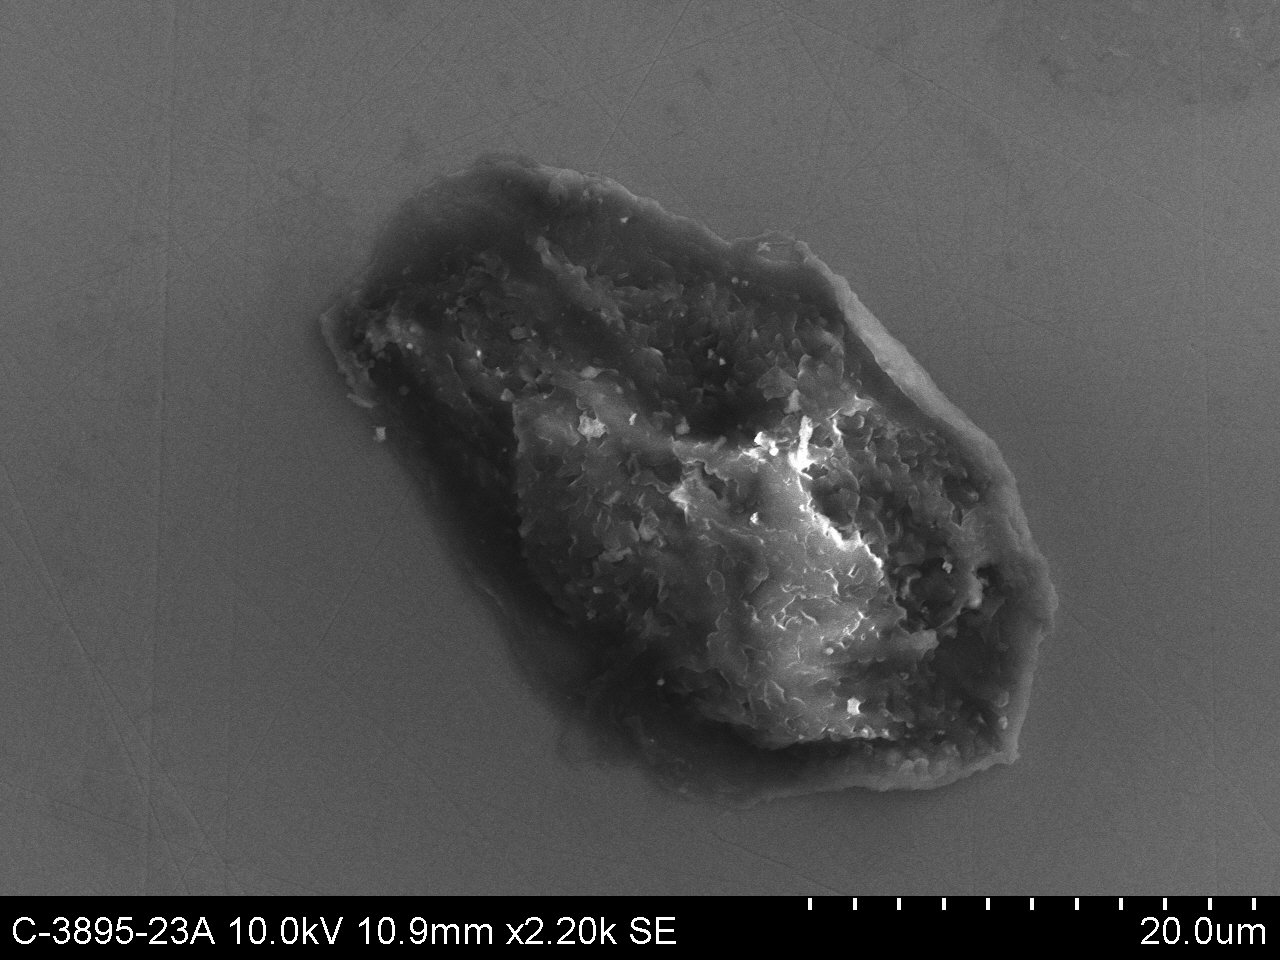
\includegraphics[width=\linewidth]{C-3895-23A_tuning_05.jpg}%{carbon_eds_sem.jpg} %{C-3895-23_02_m002.jpg}%{C-3895-23A_tuning_05.jpg}
          \end{minipage}
          \hfill
          \begin{minipage}[t]{0.49\linewidth}
            \centering
            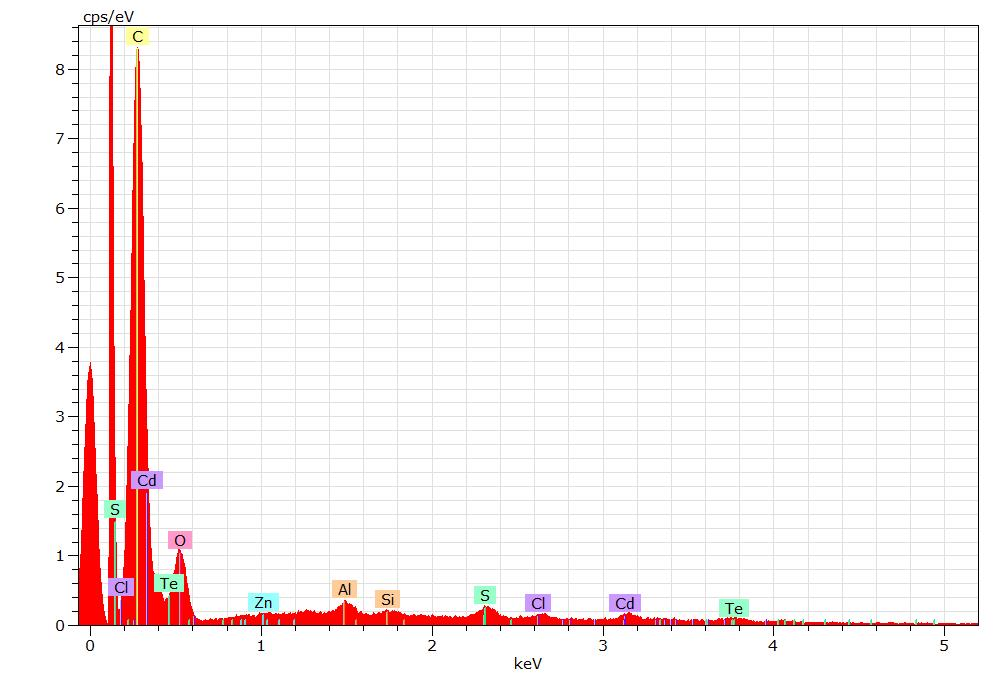
\includegraphics[width=\linewidth]{carbon_eds.jpg}
          \end{minipage}
        \caption{\Ac{sem} image of a carbon based particle at a magnification of $10000\times$ and the corresponding \ac{eds} spectrum. The spectrum shows that the particle consists mainly of carbon (\ce{C}).}\label{fig:subBa_particle_carbon}
    \end{subfigure}%
    \par\bigskip
    \begin{subfigure}[t]{\textwidth}
          \begin{minipage}[t]{0.49\linewidth}
            \centering
            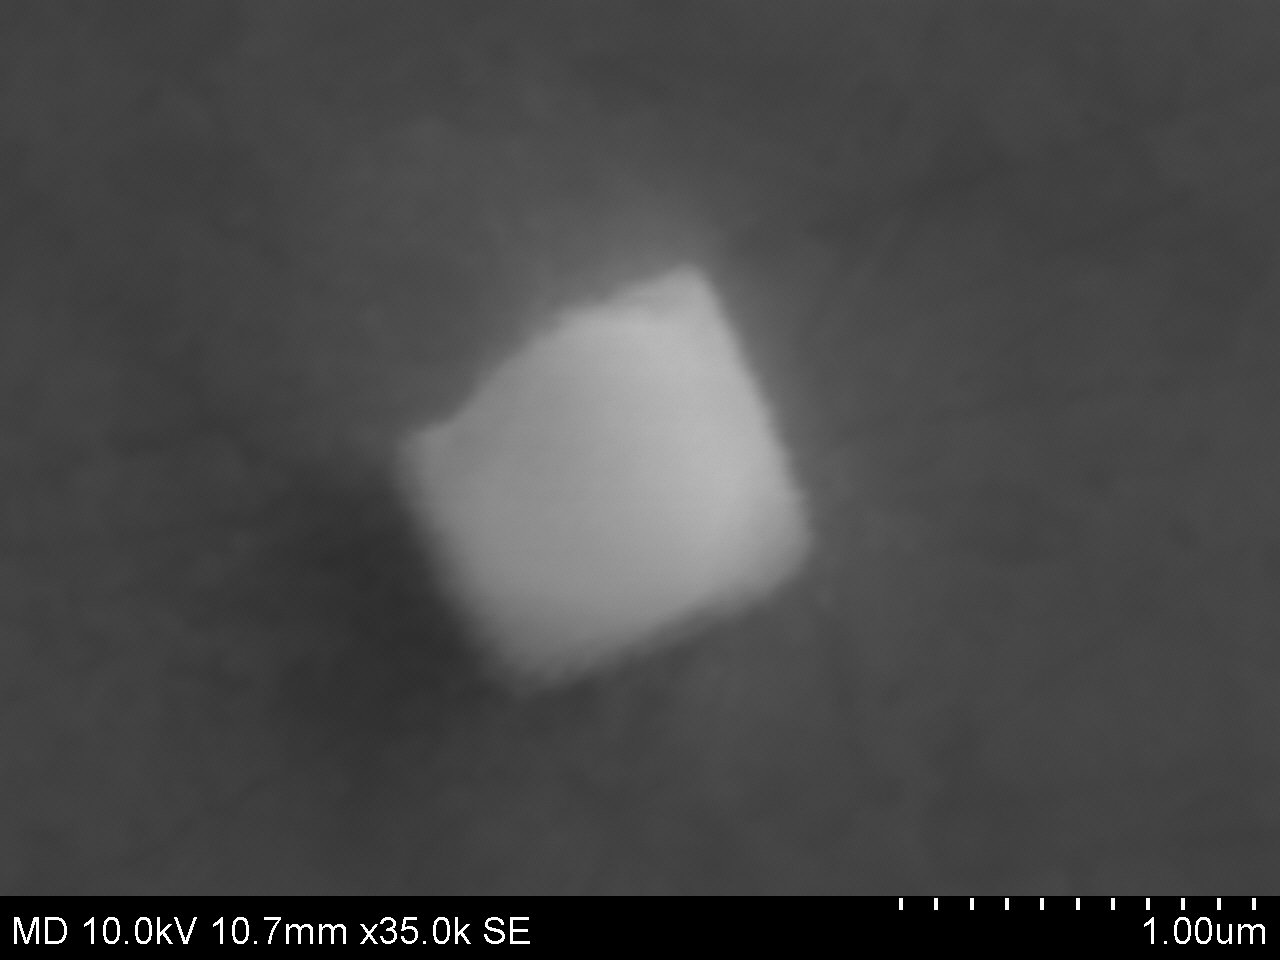
\includegraphics[width=\linewidth]{eds_NaOCl2_C-3895-23A_edx8_m007.jpg}
          \end{minipage}
          \hfill
          \begin{minipage}[t]{0.49\linewidth}
            \centering
            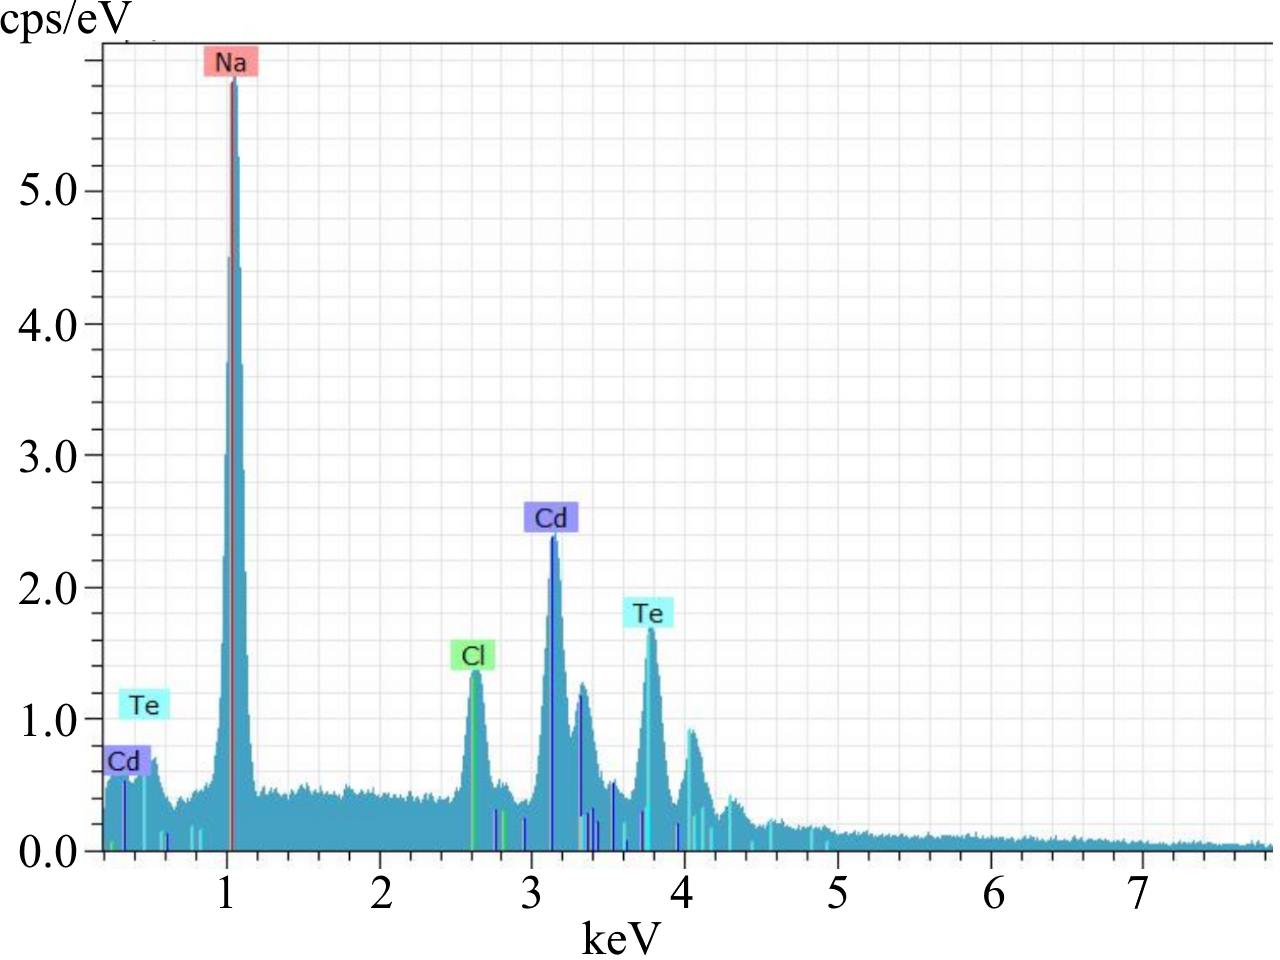
\includegraphics[width=\linewidth]{eds_NaClO2.jpg}
          \end{minipage}
    \caption{\Ac{sem} image of a \ce{NaClO} particle at a magnification of 35000$\times$ and the corresponding \ac{eds} spectrum which reveals that the particle consists of sodium (\ce{Na}), chloride (\ce{Cl}), and oxygen (\ce{O}).}\label{fig:EDS_NaClO}
    \end{subfigure}%
    \captionsetup{list=no}
    \caption{\emph{(continued)}}
\end{figure}
%
\begin{figure}[htbp]
\ContinuedFloat
    \centering
    \begin{subfigure}[t]{\textwidth}
          \begin{minipage}[t]{0.49\linewidth}
            \centering
            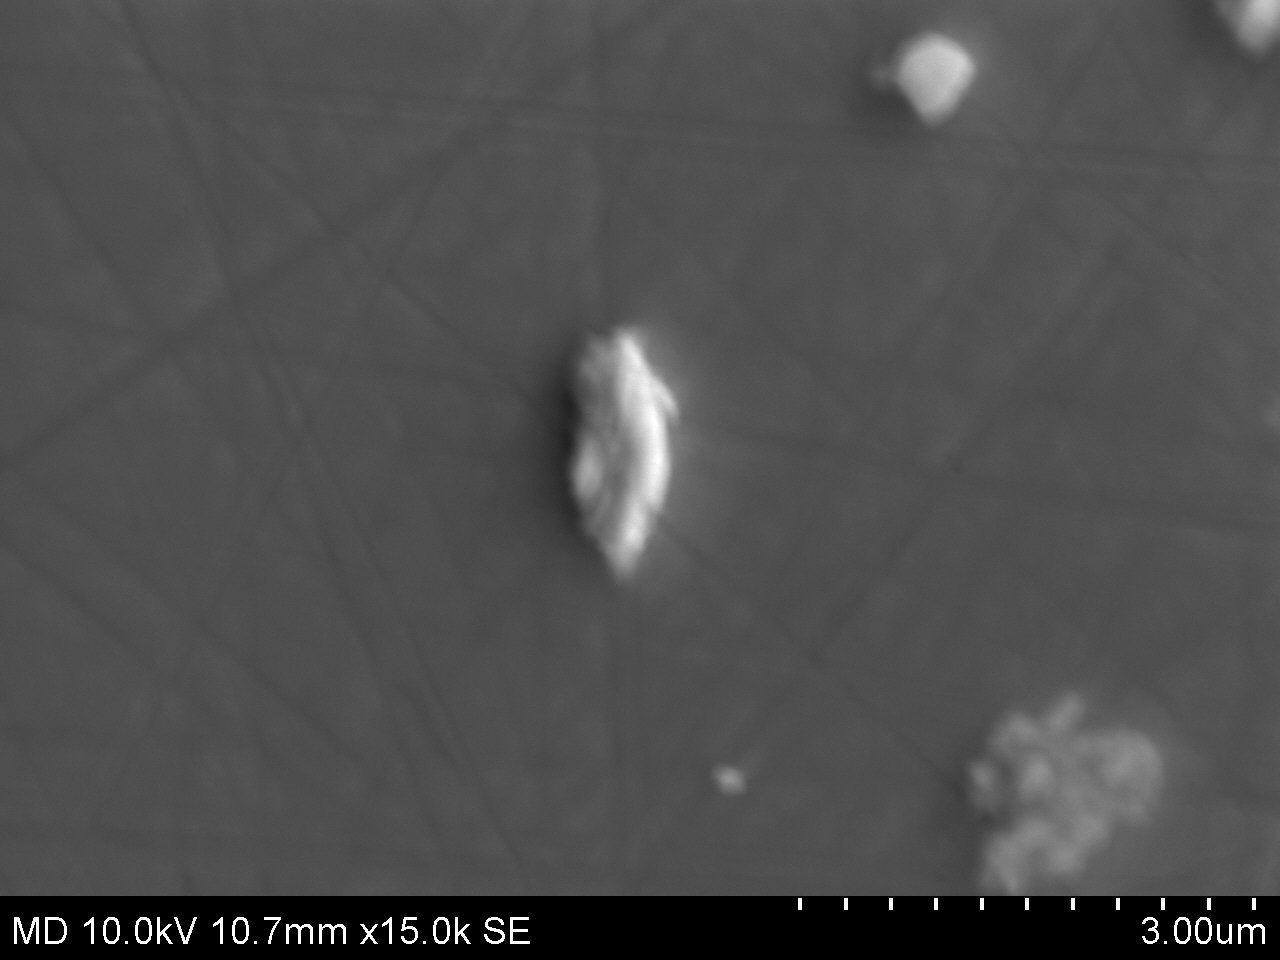
\includegraphics[width=\linewidth]{eds_Fe_C-3895-23A_edx5_m004.jpg}
          \end{minipage}
          \hfill
          \begin{minipage}[t]{0.49\linewidth}
            \centering
            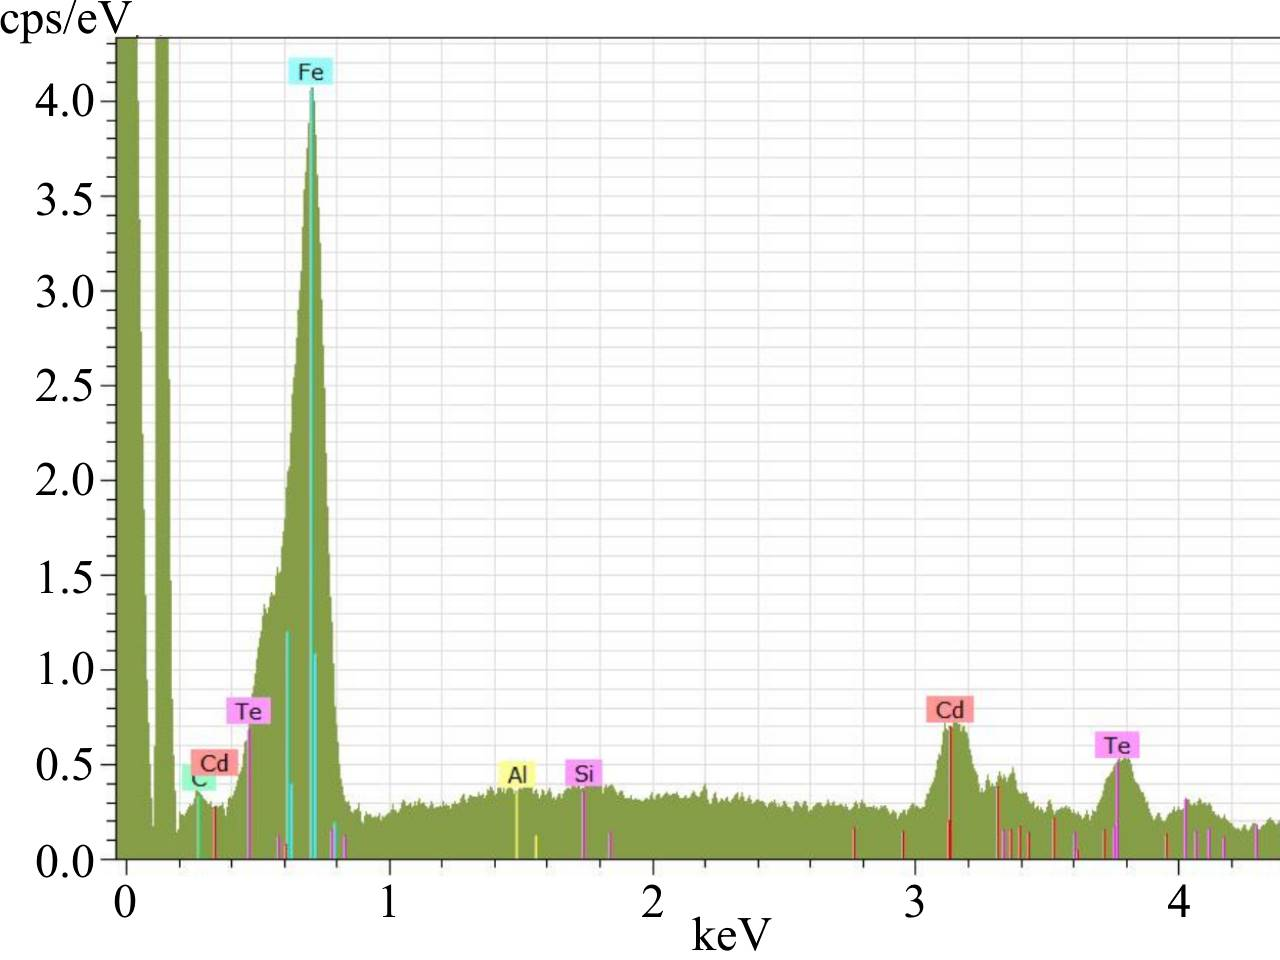
\includegraphics[width=\linewidth]{eds_Fe.jpg}
          \end{minipage}
    \caption{\Ac{sem} image of an iron particle at a magnification of $15000\times$ and the corresponding \ac{eds} spectrum which reveals that the particle consists of iron (\ce{Fe}).}\label{fig:subBa_partice_Fe}
    \end{subfigure}%
    \captionsetup{list=no}
    \caption{\emph{(continued)}}
\end{figure}

%\subsection{Voids}
%Page b1 in eds report 1-10
Irregular shaped cavities were observed all over the surface of substrate B, see Fig.~\ref{fig:SEM_C389523_voids}. The size of the cavities tends to be between \SI{5}{} and \SI{100}{\micro\metre}. \Ac{afm} gives that the cavities are between \todo{\SI{}{\nano\metre} and \SI{}{\nano\metre}} deep, see Fig.~\ref{subBa_afm_voids}. The larger ones tend to have more angular shapes than the smaller ones. The \ac{eds} spectrum in Fig.~\ref{fig:SEM_C389523_void_eds} reveals that the cavity has the same composition as the substrate surface.

\begin{figure}[htbp]
    \centering
    \begin{subfigure}[t]{\textwidth}
          \begin{minipage}[t]{0.49\linewidth}
            \centering
            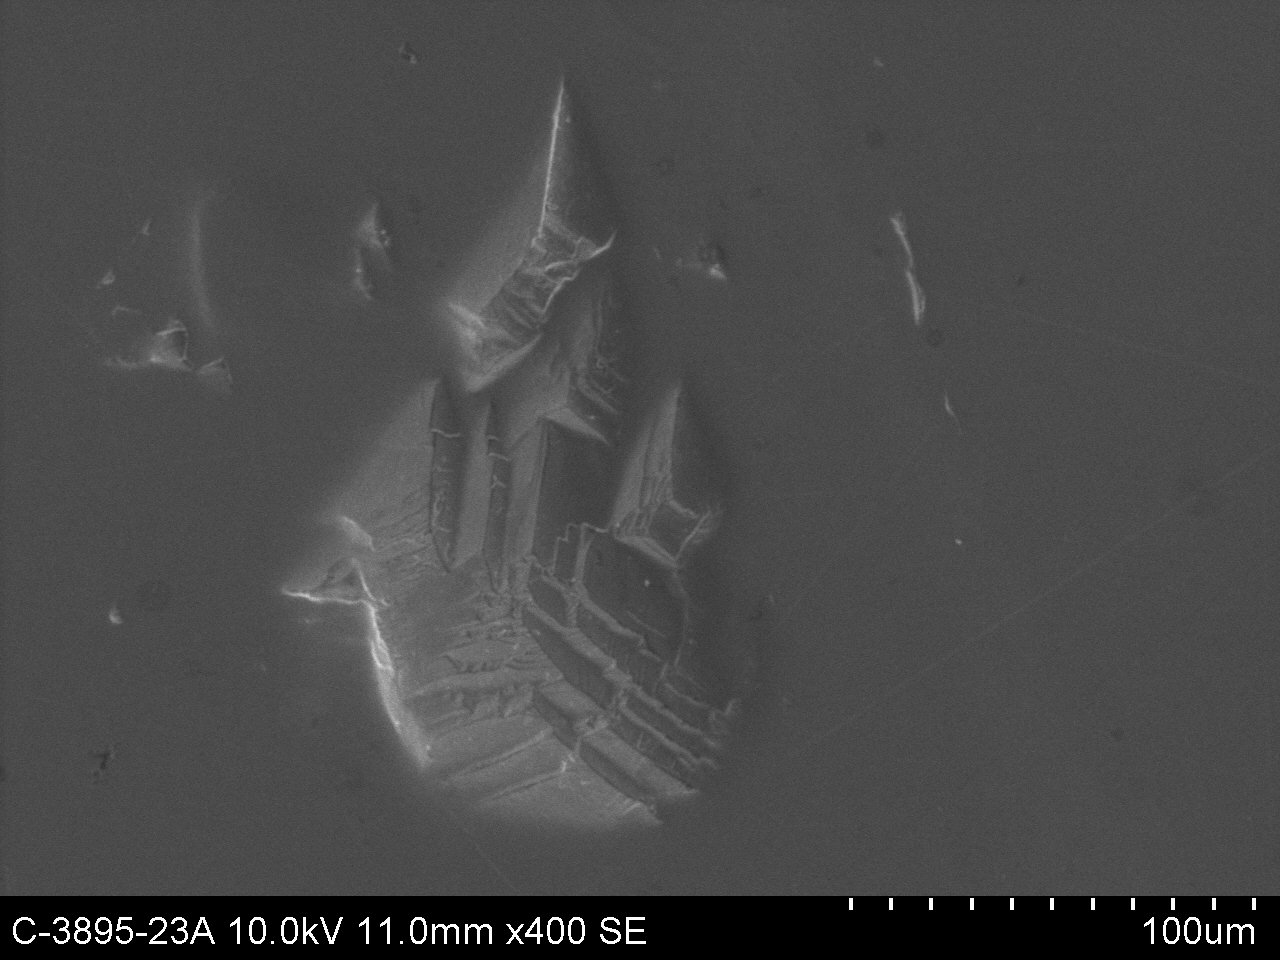
\includegraphics[width=\linewidth]{C-3895-23A_tuning_04.jpg}
          \end{minipage}
          \hfill
          \begin{minipage}[t]{0.49\linewidth}
            \centering
            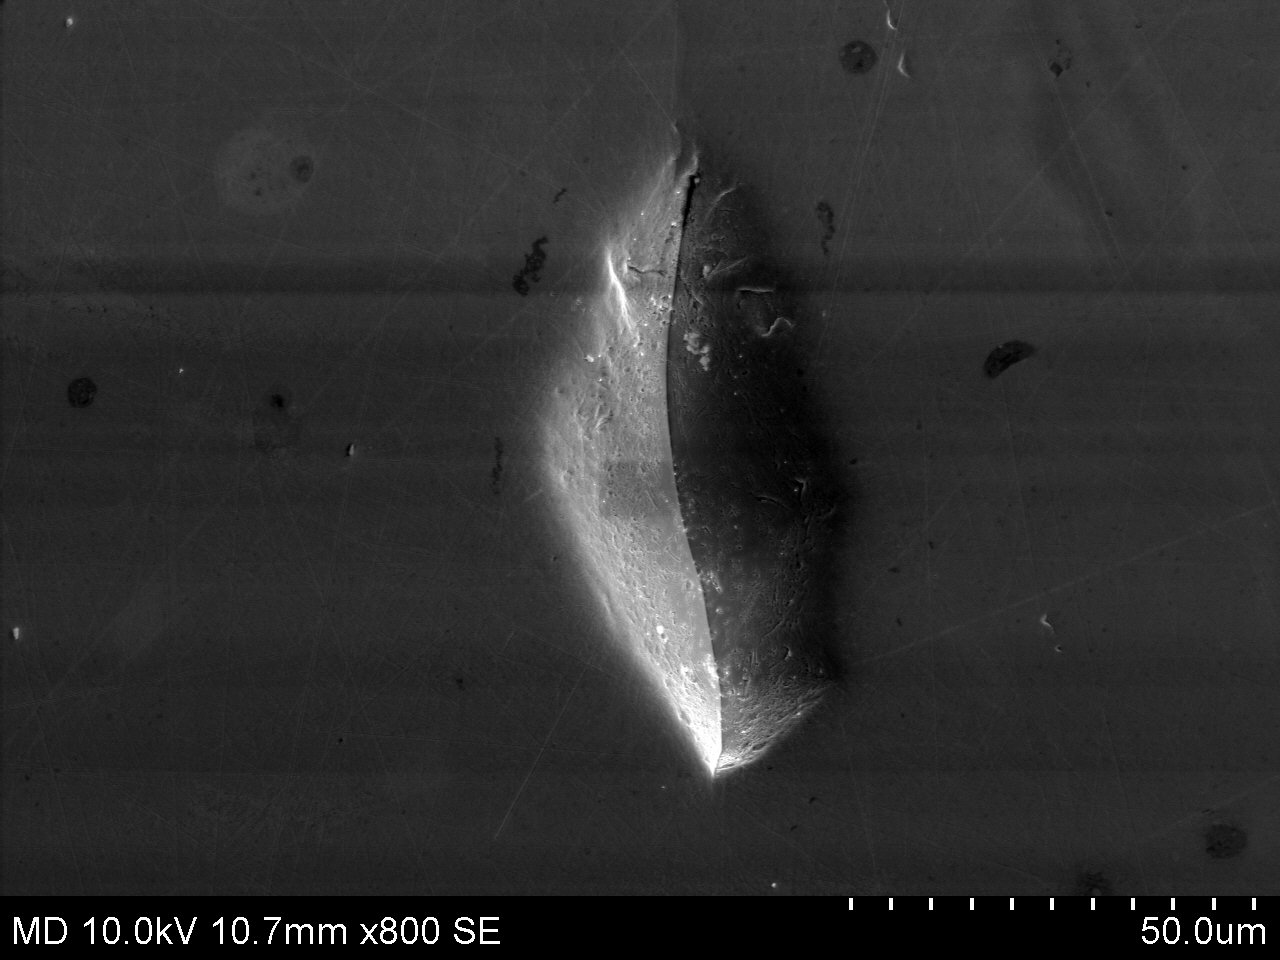
\includegraphics[width=\linewidth]{C-3895-23A_edx3_m002.jpg}
          \end{minipage}
    \caption{}\label{fig:subBa_high-temperature-voids}
    \end{subfigure}%
    \par\bigskip
    %\mySubfigure[SEM.]{0.44\linewidth}{C-3895-23A_edx7_m002.jpg}
    %\mySubfigure[SEM.]{0.44\linewidth}{C-3895-23A_edx7_m003.jpg}
    \begin{subfigure}[t]{\textwidth}
          \begin{minipage}[t]{0.49\linewidth}
            \centering
            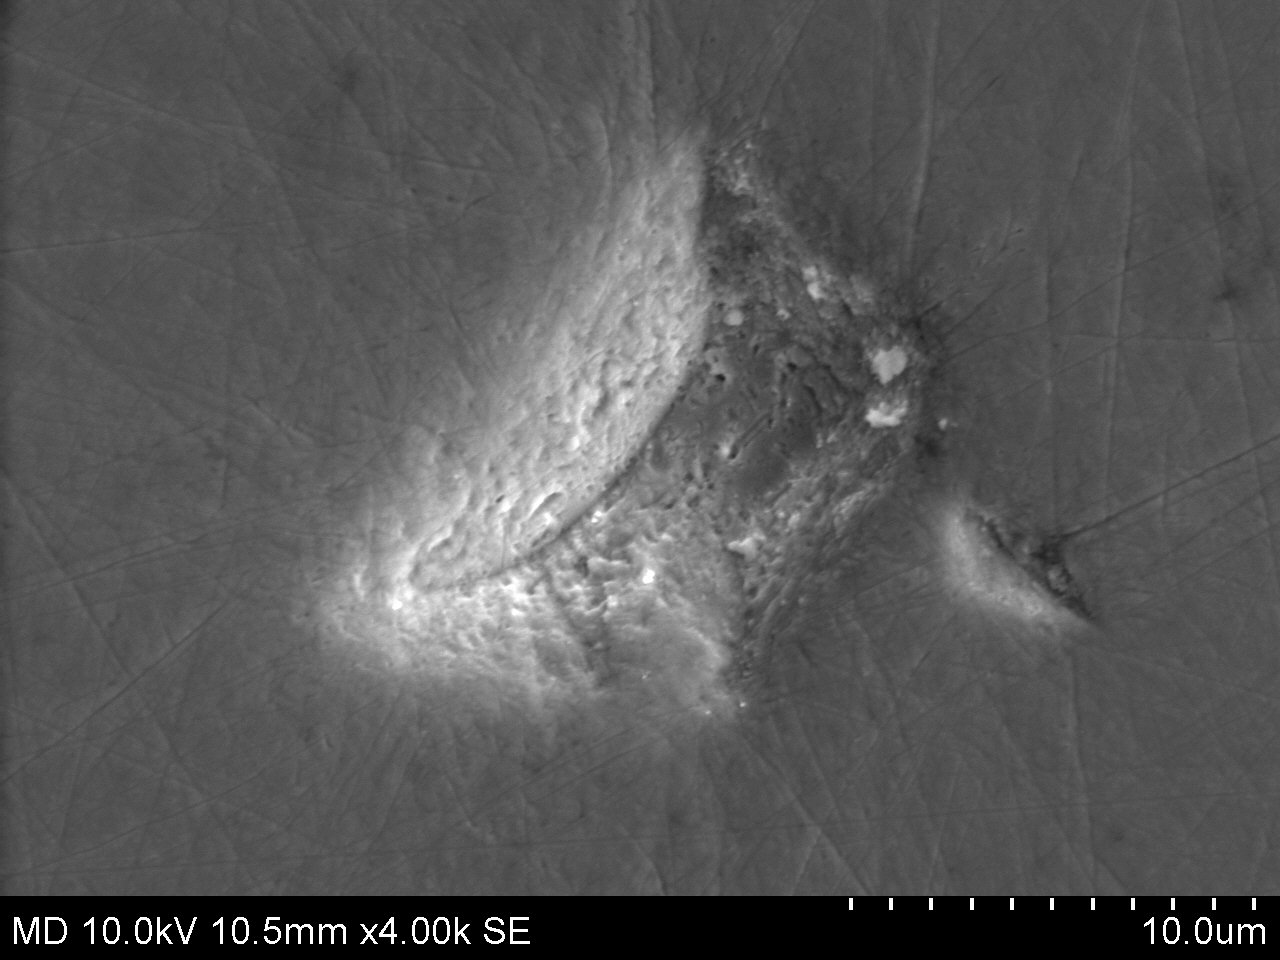
\includegraphics[width=\linewidth]{C-3895-23A_edx7_m004.jpg}
          \end{minipage}
          \hfill
          \begin{minipage}[t]{0.49\linewidth}
            \centering
            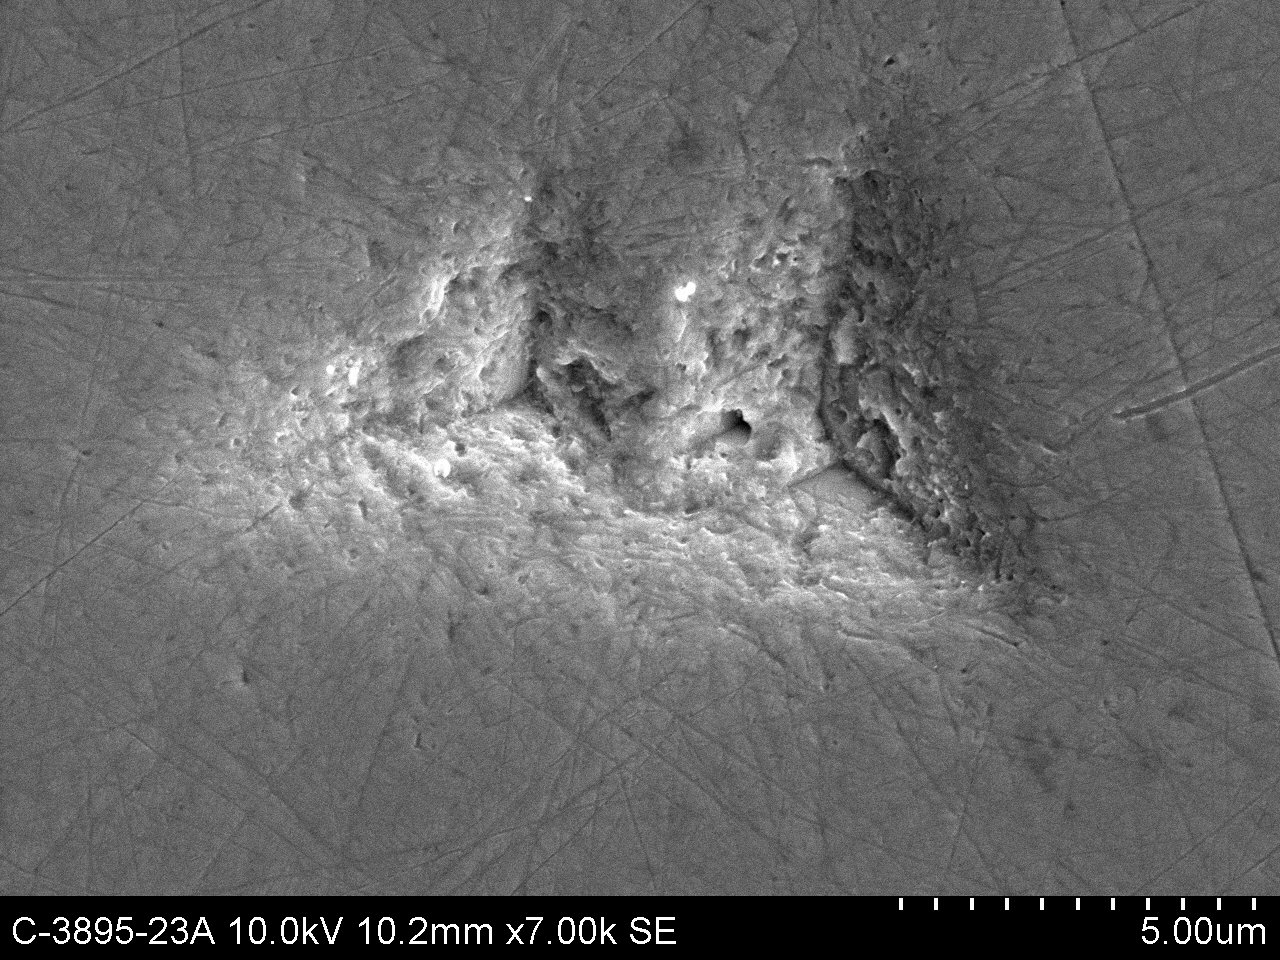
\includegraphics[width=\linewidth]{C-3895-23A_K01_detail.jpg}
          \end{minipage}
    \caption{}\label{fig:subBa_microvoids}
    \end{subfigure}%
    \caption[\Ac{sem} images of voids on substrate B.]{\Acf{sem} images of \subref{fig:subBa_high-temperature-voids} high temperature voids and \subref{fig:subBa_microvoids} microvoids on the as-received substrate B.}
    \label{fig:SEM_C389523_voids}
\end{figure}

\begin{figure}
    \begin{subfigure}[t]{0.49\linewidth}
        
\includegraphics[width=\linewidth]{unknown.png}
        \caption{}\label{fig:subBa_afm_void}
    \end{subfigure}%
    \hfill
    \begin{subfigure}[t]{0.49\linewidth}
        
\includegraphics[width=\linewidth]{unknown.png}
        \caption{}\label{fig:subBa_afm_microvoid}
    \end{subfigure}%
    \caption[\Ac{afm} measurements of void and microvoid on as-received substrate B.]{\Acf{afm} measurements of \subref{fig:subBa_afm_void} a high temperature void and \subref{fig:subBa_afm_microvoid} a microvoid on the as-received substrate B.}
    \label{fig:subBa_afm_voids}
\end{figure}

\citet{selvig2007defects} describe the irregularly shaped defects with sizes extending from \SI{10}{\micro\metre} to a few hundred microns as high temperature voids, see Fig.~\ref{fig:subBa_high-temperature-voids}, and the ones with size less than \SI{10}{\micro\metre} as microvoids, see Fig.~\ref{fig:subBa_microvoids}. These types of defects are typically formed during the growth of the material and the density is dependent on the deviation from ideal growth conditions. High temperature voids are formed at substrate temperatures higher than the \ce{Te}-phase limit, while microvoids are formed at low substrate temperature.

The void density was found to be between \SI{1e+02}{\centi\metre^{-2}} and \SI{2e+3}{\centi\metre^{-2}}. The mean void density was \SI{4e+02}{\centi\metre^{-2}} with a standard deviation of \SI{3e+02}{\centi\metre^{-2}}. A graphical representation of the void density at different locations on substrate B can be seen in Fig.~\ref{fig:subBa_densityData_void}.

\begin{figure}[htbp]
    \centering
        \mySubfigure{0.403\linewidth}{subBa_densityData_voids.png}[fig:subBa_densityData_void_map]
        \hfill
        \mySubfigure{0.577\linewidth}{C-3895-23A_A01_x060.jpg}[fig:subBa_densityData_void_sem]
    \caption[Map of the void density on the as-received substrate B.]{\subref{fig:subBa_densityData_void_map} A map of the void density at 36 different locations on the as-received $\SI{30}{\milli\metre}\times\SI{30}{\milli\metre}$ substrate B. The void density was observed to vary between \SI{1e+02}{\centi\metre^{-2}} and \SI{2e+3}{\centi\metre^{-2}}. \subref{fig:subBa_densityData_void_sem} An image from the upper right corner of the grid where the void density is highest.}
    \label{fig:subBa_densityData_void}
\end{figure}

The microvoid density was found to be between \SI{2e+03}{\centi\metre^{-2}} and \SI{2e+4}{\centi\metre^{-2}}. The mean microvoid density was \SI{6e+03}{\centi\metre^{-2}} with a standard deviation of \SI{5e+03}{\centi\metre^{-2}}. A graphical representation of the microvoid density at different locations on substrate B can be seen in Fig.~\ref{fig:subBa_densityData_microvoid}.
%Voids: Minimum = 1.28e+02. Maximum = 1.91e+03. Mean = 4.20e+02. Standard deviation = 3.26e+02.
%Microvoids: Minimum = 2.21e+03. Maximum = 2.21e+04. Mean = 6.09e+03. Standard deviation = 5.06e+03

\begin{figure}[htbp]
    \centering
        \mySubfigure{0.403\linewidth}{subBa_densityData_microvoids.png}[fig:subBa_densityData_microvoid_map]
        \hfill
        \mySubfigure{0.577\linewidth}{C-3895-23A_A11_x500.jpg}[fig:subBa_densityData_microvoid_sem]
    \caption[Map of the microvoid density on the as-received substrate B.]{\subref{fig:subBa_densityData_microvoid_map} A map of the microvoid density at 36 different locations on the as-received $\SI{30}{\milli\metre}\times\SI{30}{\milli\metre}$ substrate B. The microvoid density was observed to vary between \SI{2e+03}{\centi\metre^{-2}} and \SI{2e+4}{\centi\metre^{-2}}. \subref{fig:subBa_densityData_microvoid_sem} An image from the upper right corner of the grid where the microvoid density is highest.}
    \label{fig:subBa_densityData_microvoid}
\end{figure}

%\subsubsection{Type B.I}
%Page 5-6 in eds report 1-10
Fig.~\ref{fig:SEM_B_particulates} shows \ac{sem} images of large pieces of material on the substrate surface. The size of the pieces is typically between \SI{50}{\micro\metre} and \SI{100}{\micro\metre}.

\begin{figure}[htbp]
    \centering
          \begin{minipage}[t]{0.49\linewidth}
            \centering
            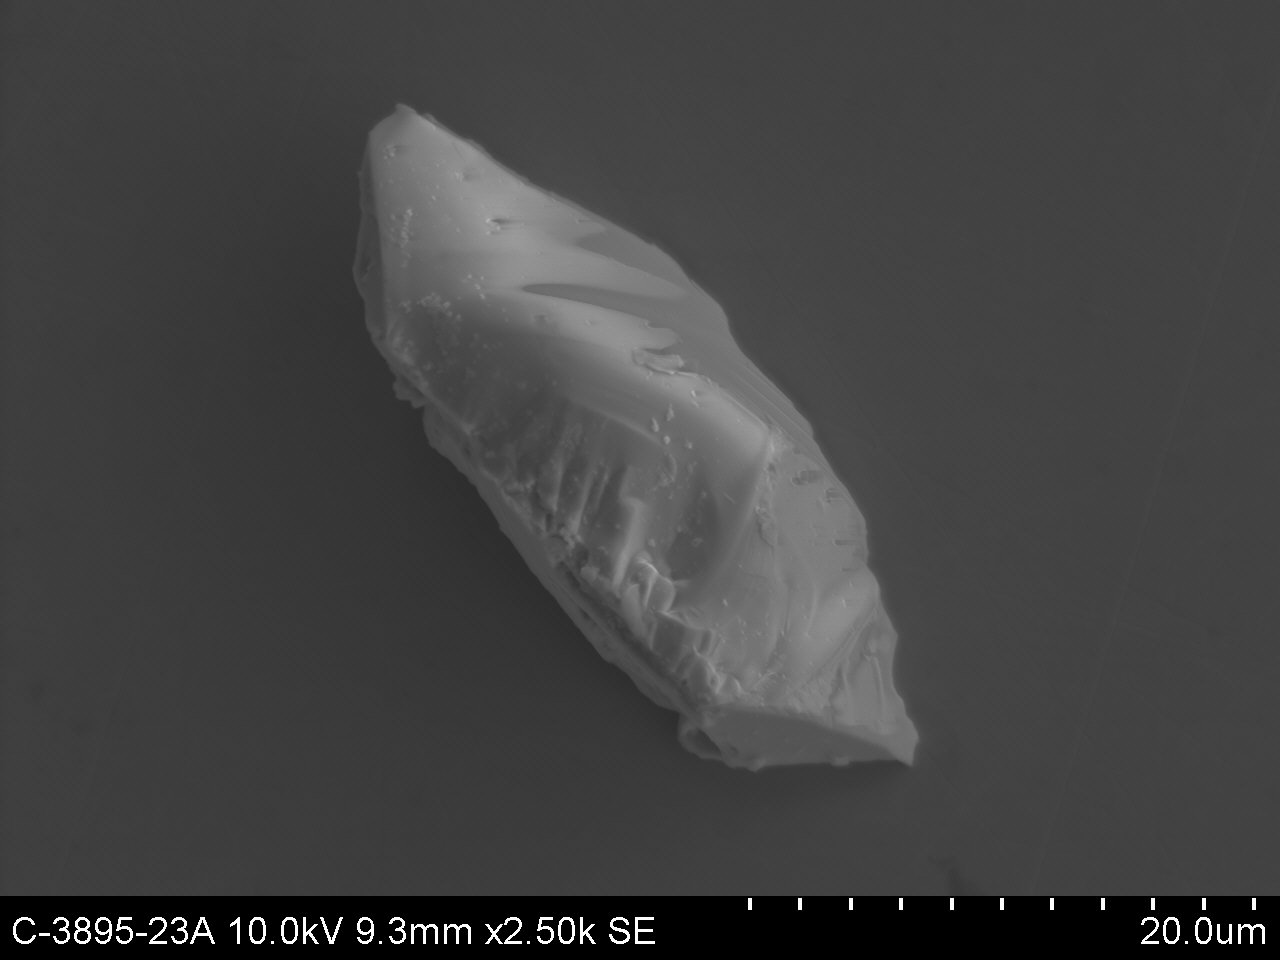
\includegraphics[width=\linewidth]{C-3895-23_03.jpg}
          \end{minipage}
          \hfill
          \begin{minipage}[t]{0.49\linewidth}
            \centering
            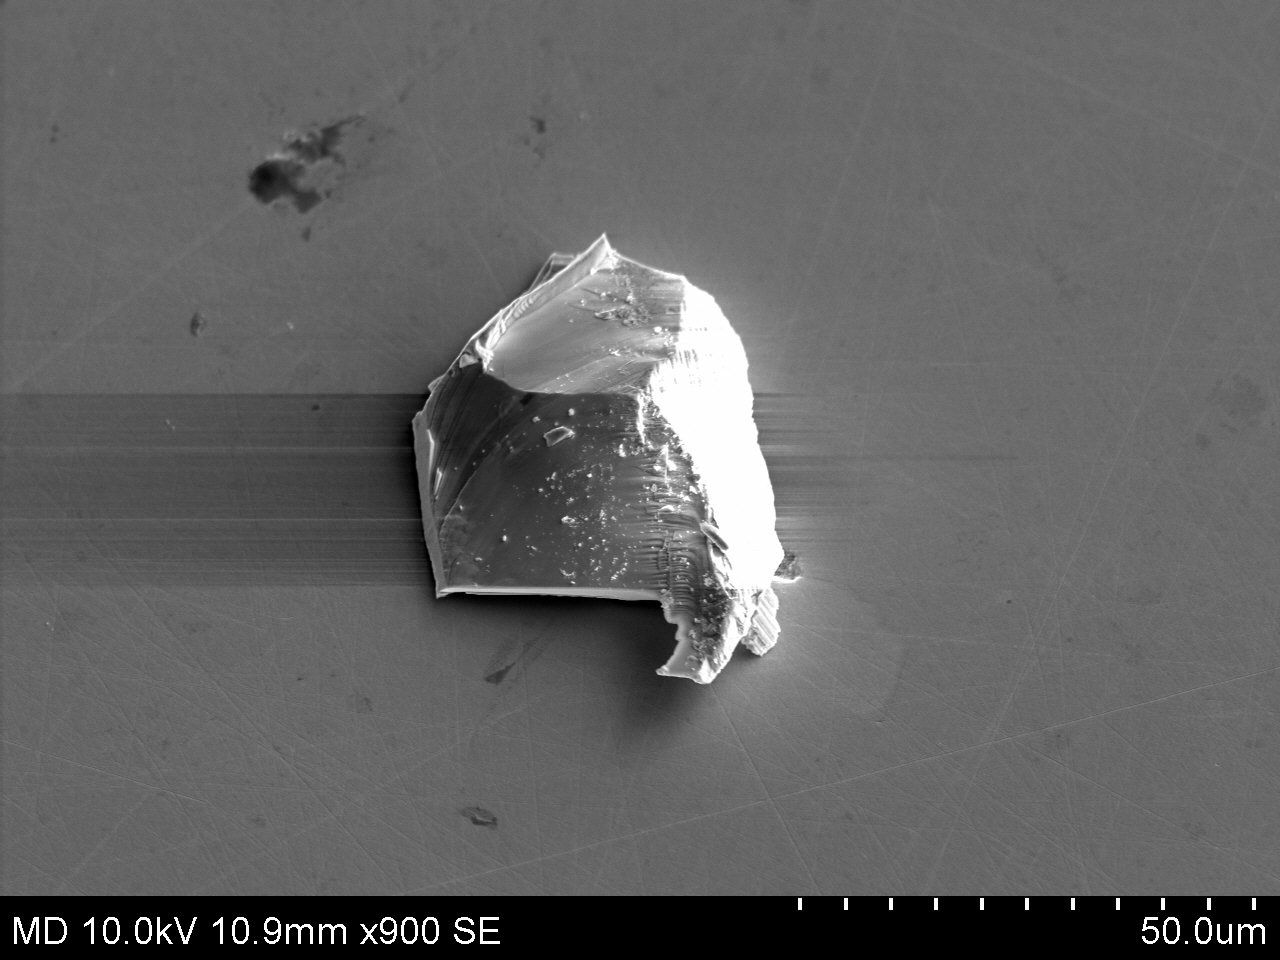
\includegraphics[width=\linewidth]{C-3895-23A_edx1_m006.jpg}
          \end{minipage}
        \caption[\Ac{sem} images of a particle on substrate B.]{\Acf{sem} images of a particle on substrate B.}\label{fig:SEM_B_particulates}  
\end{figure}

By comparing the \ac{eds} spectrum of the particle with the spectrum of the substrate surface, see Fig.~\ref{fig:SEM_B_particulates_eds}, it is seen that they are essentially the same. This indicates that the pieces consist of the same material as the substrate and that they could be debris from the cutting of the substrate.

%\subsubsection{Type B.III - Residual Polishing Grit}
Fig.~\ref{fig:subBa_polishing-grit_area1} displays an area on the surface where there are accumulations of small particles. Fig.~\ref{fig:subBa_polishing-grit_area2} display one of these accumulations at greater magnification. The large particles appear to be agglomerations of smaller particles that are between \SI{50}{\nano\metre} and \SI{100}{\nano\metre} in diameter. The typical width of the particle agglomerations is \SI{0.5}{}-\SI{3}{\micro\metre}. The attraction between the small particles can be explained by electrostatic attractive forces between the particles due to different surface charge \citep{allen2001review}.

\begin{figure}[htbp]
    \centering
        \mySubfigure[Magnification of 200$\times$.]{0.49\linewidth}{SEM_C-3895-23A_a_m001.jpg}[fig:subBa_polishing-grit_area1]
        \hfill
        \mySubfigure[Magnification of 15000$\times$.]{0.49\linewidth}{C-3895-23Ab_m003.jpg}[fig:subBa_polishing-grit_area2]
    \caption[\Ac{sem} images of particles on substrate B.]{\Acf{sem} images of an accumulation of particles on substrate B.}\label{fig:subBa_polishing-grit_area}
\end{figure}

An \ac{eds} spectrum of the particle reveals that the piece is composed of alumina oxide, \ce{Al2O3}, also known as alumina, see Fig.~\ref{fig:subBa_polishing-grit_alumina}. The corresponding \ac{sem} image of residual polishing grit is shown next to the spectrum. The presence of alumina can be explained by the frequent use of alumina as an abrasive in polishing slurries for semiconducting material.

The slurry polishes and flattens the substrate through chemical and mechanical action. The alumina particles in the slurry are suspended throughout the bulk of the medium because of the negative charges that are incorporated on the alumina particle surface and make the particles repel each other. This can explain the observations of agglomerations of alumina. 
%Residual polishing grit can be observed at different locations on the substrate. \mycomment{density?}

Fig.~\ref{fig:subBa_polishing-grit_silica} displays an area on the surface where there are an accumulation particles that look similar to the alumina agglomerations. The largest particle in the image has a diameter of \SI{600}{\nano\metre}. An \ac{eds} spectrum of the particle reveals that the piece is composed of silicon oxide, \ce{SiO2}, also known as silica. As mentioned, silica is a frequently used abrasive in polishing slurry.

%\subsubsection{Type B.IV}
Fig.~\ref{fig:subBa_particle_carbon} shows a \ac{sem} image of a dark particle and the corresponding \ac{eds} spectrum. The typical size of these particles is between \SI{20}{} and \SI{30}{\micro\metre}. The \ac{eds} spectrum of this particle shows a high intensity from the carbon signal. The particles could be residue from mounting wax, which is used to hold the substrate while it is being cut and polished. There are some small peaks from silicon and aluminium as well, but these are probably from the residual polishing grit that can be seen in on the surface of the carbon-based particle.
%Page 8+12 in eds report 1-10

%\subsubsection{Type B.IV - \ce{NaClO}}
An area with lots of circular particles with diameter between \SI{100}{\nano\metre} and \SI{1}{\micro\metre} is observed near one of the edges of substrate B, see Fig.~\ref{fig:eds_NaOCl_overview}. The area is separated from the rest of the substrate by a dark borderline. An \ac{eds} spectrum of one particle with diameter of \SI{1}{\micro\metre}, see Fig.~\ref{fig:EDS_NaClO}, reveals that the particle consists of \ce{Na} and \ce{Cl}. The particles could be \ce{NaClO} which is used after polishing as a standard cleaner to remove polishing slurry particles \citep{benson2015as-received}. The dark borderline was not possible to get quantified with \ac{eds}, but it could be a residue of the cleaning solution.

\begin{figure}
    \centering
    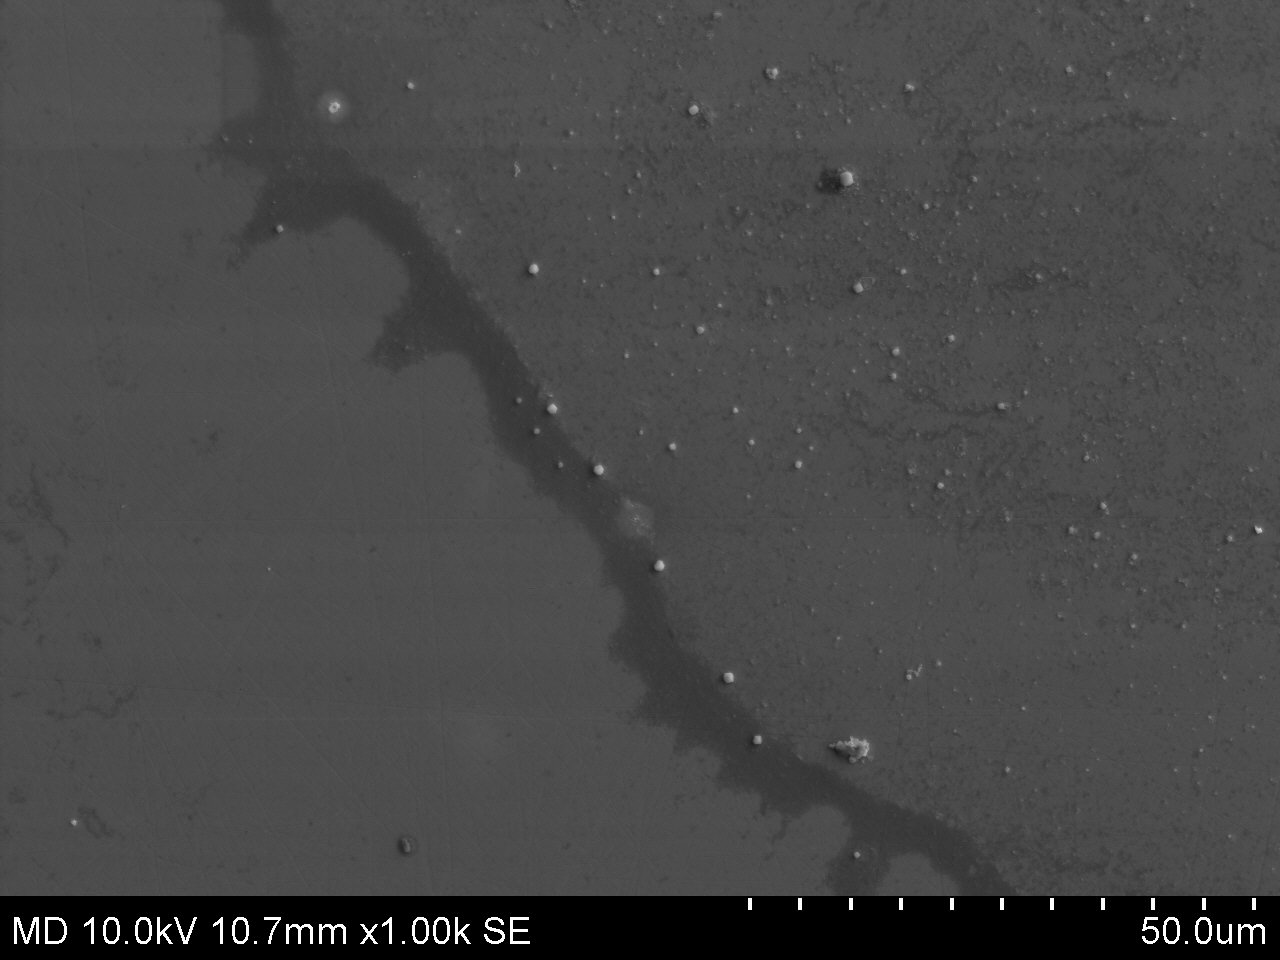
\includegraphics[width=0.48\linewidth]{eds_NaOCl_overview_C-3895-23A_edx8_m008}
    \caption{Scanning electron microscopy (SEM) image of particles of a particle on substrate B taken at a magnification of 1000$\times$.}
    \label{fig:eds_NaOCl_overview}
\end{figure}

%\subsection{Type B.V - Iron particulates}
A small particle that is \SI{1.5}{\micro\metre} long and \SI{0.6}{\micro\metre} wide can be seen in Fig.~\ref{fig:subBa_partice_Fe} with its corresponding \ac{eds} spectrum. The \ac{eds} spectrum of the particle reveals that the particle consists mainly of \ce{Fe}. Iron is a potential contaminate in polishing grit slurry, but it could also originate in cross-contamination from the polishing of other semiconductors, i.e. \ce{InP} \citep{benson2015as-received}.

\subsection{Circular stains}
Fig.~\ref{fig:subB_stains} shows four typical stains that can be observed with \ac{sem}. One type of stain can be observed in Fig.~\ref{fig:EDX_C-3895-23Ad_m001} and Fig.~\ref{fig:EDX_C-3895-23A_edx1_m005}. This type of stain is recognised by having a bright background with a darker centre in one part of the stain. The size of the bright stains varies from \SI{30}{\micro\metre} to \SI{150}{\micro\metre}. The density of this type of stain was estimated from the \ac{sem} grid map to be \SI{2e2}{\centi\metre^{-2}}. One theory  is that the stains could be residue from the evaporation of a droplet on the surface, and that the centre of the stain consists of the impurities that have been carried by the surface tension of the droplet. 

The stain seen in Fig.~\ref{fig:EDX_C-3895-23A_edx1_m003} appears dark in the \ac{sem} image and stains similar to this have sizes from \SI{8}{\micro\metre} to \SI{15}{\micro\metre}. The density of these stains was estimated from the \ac{sem} grid map to be \SI{1e3}{\centi\metre^{-2}}. The last type of stain appears as a dark shadow on the substrate surface when observed in \ac{sem}, see Fig.~\ref{fig:EDX_C-3895-23A_edx1_m016}. The typical size of stains like this is \SI{10}{} to \SI{50}{\micro\metre} and density of these stains was estimated to be \SI{1e4}{\centi\metre^{-2}}. The observed stains have in common that they do not contribute with any additional signal to the \ac{eds} spectrum due to their thin layer on the surface, and therefore has it not been possible to identify exactly what they are. 
%Page 11 in eds report 1-10
\begin{figure}[htbp]
    \centering
    \mySubfigure[Magnification of 1500$\times$.]{0.48\linewidth}{C-3895-23A_edx1_m001.jpg}[fig:EDX_C-3895-23Ad_m001]
    \mySubfigure[Magnification of 900$\times$.]{0.48\linewidth}{C-3895-23A_edx1_m005.jpg}[fig:EDX_C-3895-23A_edx1_m005]
    \par\bigskip
    \mySubfigure[Magnification of 3500$\times$.]{0.48\linewidth}{C-3895-23A_edx1_m003.jpg}[fig:EDX_C-3895-23A_edx1_m003]
    \mySubfigure[Magnification of 1000$\times$.]{0.48\linewidth}{C-3895-23A_edx1_m016.jpg}[fig:EDX_C-3895-23A_edx1_m016]
    \caption[\Ac{sem} images of stains on substrate B.]{\Acf{sem} images of stains on substrate B.}
    \label{fig:subB_stains}
\end{figure}

%%=========================================

%%=========================================
%\section{AFM Study of As-Received Substrate B}
\subsection{Surface Scratches and Roughness}
The surface of substrate B has been subjected to a rough polish and scratches stemming from the polishing can be seen on the surface. The scratches are typically between \SI{10}{\nano\metre} and \SI{100}{\nano\metre} wide, as seen in Fig.~\ref{fig:C-3895-23Ad_m002}, but some large scratches located near the edges are as wide as \SI{1}{\micro\metre}, as seen in Fig.~\ref{fig:C-3895-23A_J08_detail}. The largest scratches are not evenly distributed as the polishing scratches, which could be caused by substrate handling tools, i.e. tweezers. The surface scratches on substrate B are most likely deeper than those on substrate A since they are visible on the dark field images of substrate B. Substrate B needs a final polishing before growth to get rid of the scratches.
\begin{figure}[htbp]
    \centering
    \mySubfigure[SEM image at a magnification of 15000$\times$.]{0.48\linewidth}{C-3895-23Ad_m002.jpg}[fig:C-3895-23Ad_m002]
    \mySubfigure[SEM image at a magnification of 2000$\times$.]{0.48\linewidth}{C-3895-23A_J08_detail.jpg}[fig:C-3895-23A_J08_detail]
    \caption[SEM images of scratches on substrate B.]{Scanning electron microscopy (SEM) images of scratches on substrate B.}
    \label{fig:SEM_C389523_scratches}
\end{figure}

The surface topography of the as-received substrate B as seen in \ac{afm}, is shown in Fig.~\ref{fig:subBa_afm}. The \ac{rms} roughness of substrate B is \SI{\sim 4}{\nano\metre} at the centre and \SI{\sim 5}{\nano\metre} around the edges. This indicates that the substrate has large scratches and that it is less superior than substrate A. The \ac{czt} substrate surfaces are easily damaged by surface scratches caused by mechanical lapping \citep{egan2009scanning}. As can be observed in all the \ac{afm} images, the final polishing step has left scratches on the surface. The largest polishing scratches on substrate B are \SI{0.3}{\micro\metre} wide and \SI{15}{\nano\metre} deep.

\begin{figure}[htbp] % trim = left lower right upper
    \centering
    \begin{subfigure}[t]{0.3\linewidth}
    \centering
        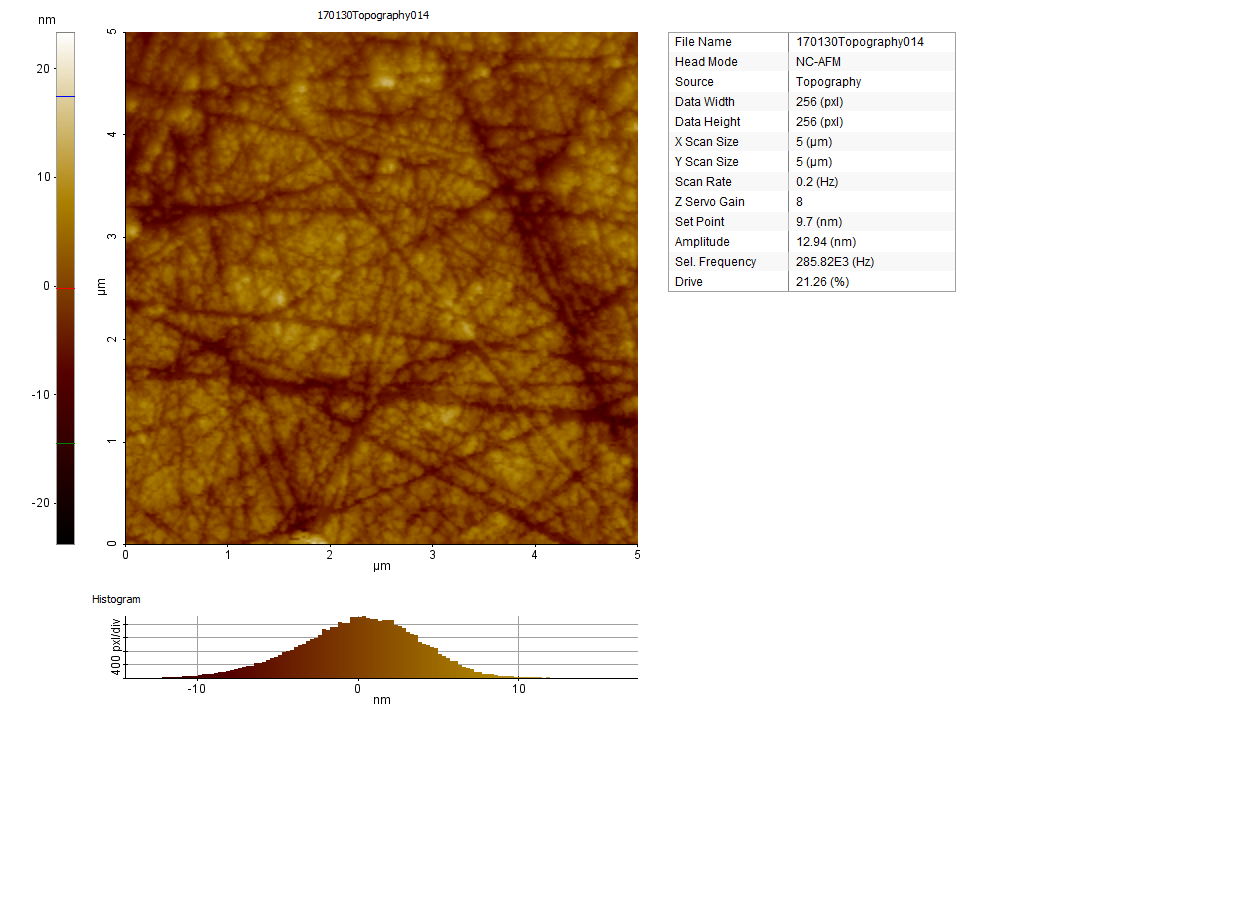
\includegraphics[width=\linewidth,trim={0cm 12cm 21cm 0cm},clip]{170130Topography014.png}
        \caption{}\label{fig:subBa_afm_centre}
    \end{subfigure}
    \hfill
    \begin{subfigure}[t]{0.3\linewidth}
    \centering
        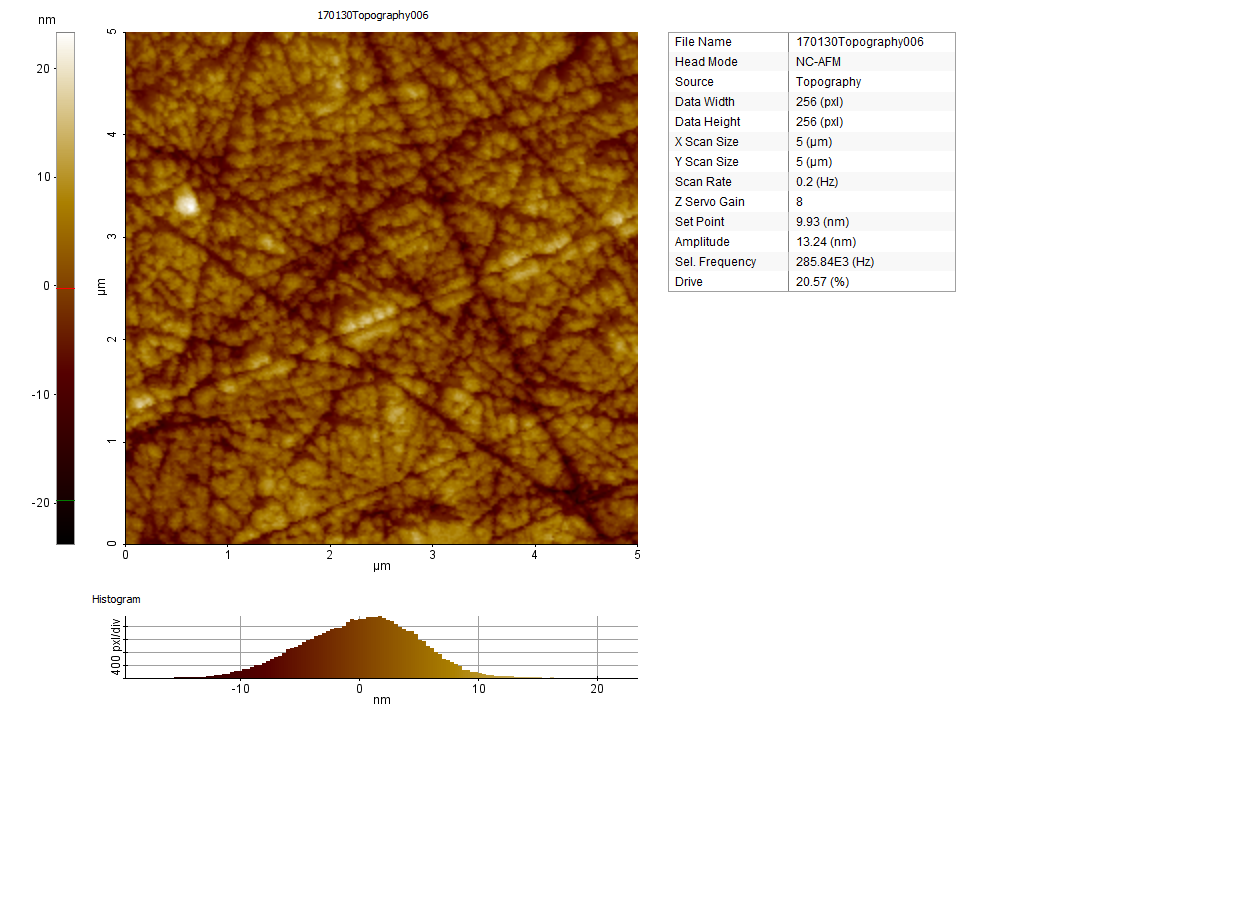
\includegraphics[width=\linewidth,trim={0cm 12cm 21cm 0cm},clip]{170130Topography006.png}
        \caption{}\label{fig:subBa_afm_edge}
    \end{subfigure}
    \hfill
    \begin{subfigure}[t]{0.3\linewidth}
    \centering
        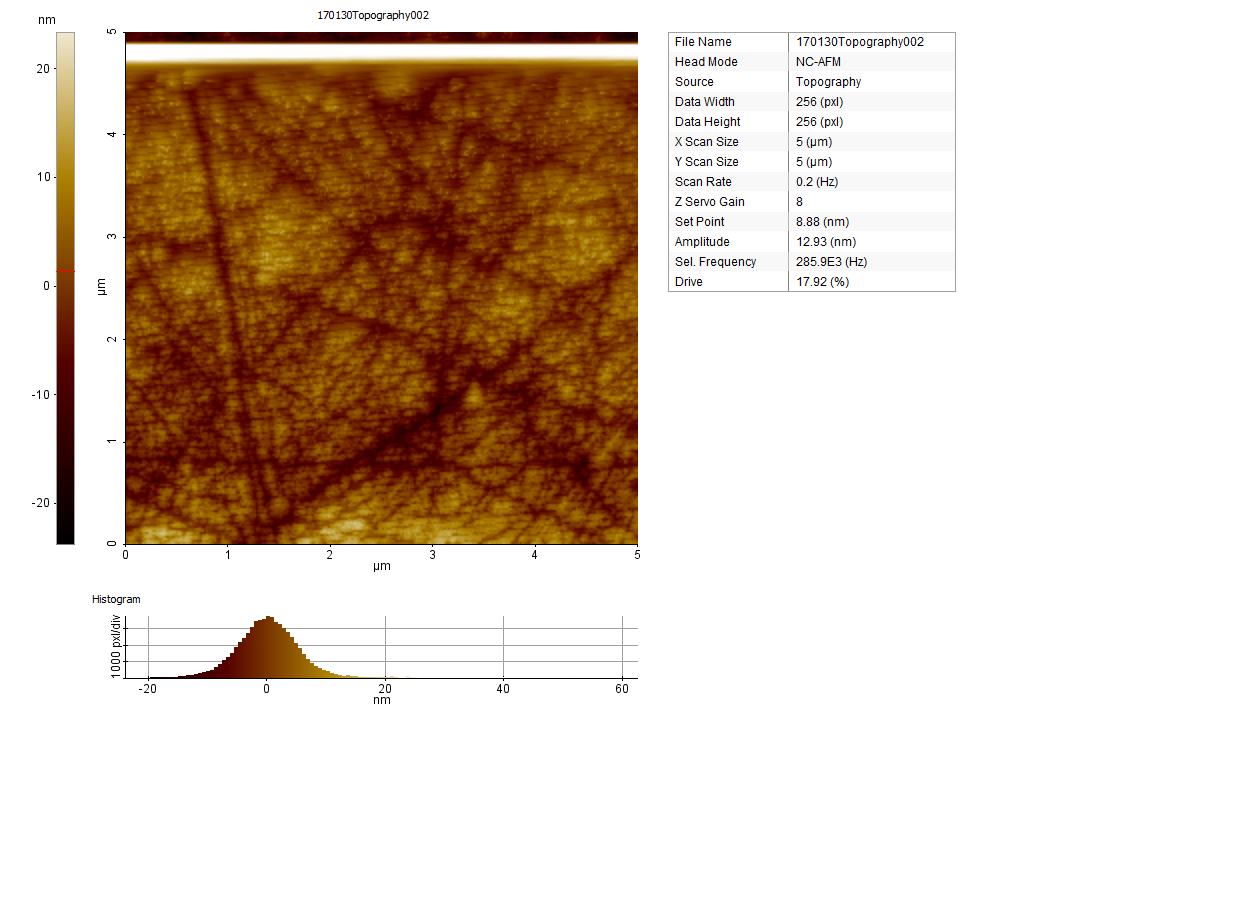
\includegraphics[width=\linewidth,trim={0cm 12cm 21cm 0cm},clip]{170130Topography002.png}
        \caption{}\label{fig:subBa_afm_corner}
    \end{subfigure}
    \caption[\Ac{afm} of as-received substrate B.]{\Acf{afm} measurements of the as-received substrate B. Images of $\SI{5}{\micro\metre}\times\SI{5}{\micro\metre}$ areas are taken at three different locations on the substrate surface: \subref{fig:subBa_afm_centre} near the centre, \ac{rms} roughness \SI{3,7}{\nano\metre}; \subref{fig:subBa_afm_edge} near the left edge, \ac{rms} roughness \SI{4,8}{\nano\metre}; and \subref{fig:subBa_afm_corner} near the upper left corner, \ac{rms} roughness \SI{4,8}{\nano\metre}. The bright line near the top of the image is due to the tip losing track of the surface.}\label{fig:subBa_afm}
\end{figure} % AFM, substrate B, as-received.

%%=========================================
%\section{Near-IR of As-Received Substrate B}

%%=========================================
\subsection{Impurity Analysis}

\Ac{eds} impurity analysis was performed on the as-received substrate B. Three locations on the surface -- the centre, the edge, and the corner -- were analysed. The results of this analysis can be seen in Table~\ref{tab:subBa_eds_analysis}. The only elements found above the \ac{eds} detection limit, in addition to \ce{Cd}, \ce{Zn}, and \ce{Te}, were \ce{Al}, \ce{Si}, \ce{C}, and \ce{O}. The relative concentrations of \ce{Cd}, \ce{Zn}, and \ce{Te} had an error of less than one percentage point from the expected value of \SI{48}{\atomic\percent} cadmium, \SI{2}{\atomic\percent} zinc and \SI{50}{\atomic\percent} tellurium.

\begin{table}[htbp]
    \centering
    \caption[\Ac{eds} impurity analysis of the as-received substrate B.]{Results of the \acf{eds} impurity analysis at three different locations on the $30\times30$ \SI{}{\milli\metre^2} as-received (111)B \ac{czt} substrate B (atomic concentration \%). The X-ray signal is acquired from $\SI{1270}{\micro\metre}\times\SI{890}{\micro\metre}$ areas near the centre, upper edge, and upper left corner.}\label{tab:subBa_eds_analysis}
    \begin{tabu} to 1.0\textwidth { X[1.85,r] X[1.125,c] X[1.125,c] X[1.125,c] X[1.125,c] X[1.125,c] X[1.125,c] X[1.125,c] }
    \hline
         & \textbf{\ce{Te}} (at.\%) & \textbf{\ce{Cd}} (at.\%) & \textbf{\ce{Zn}} (at.\%) & \textbf{\ce{Al} } (at.\%) & \textbf{\ce{Si}} (at.\%) & \textbf{\ce{C}} (at.\%) & \textbf{\ce{O}} (at.\%) \\ % \textbf{$X$} (\SI{}{\milli\metre}) &  \textbf{$Y$} (\SI{}{\milli\metre})
        \hline
        Near centre & \SI{45.88}{} & \SI{45.35}{} & \SI{2.13}{} & \SI{0.18}{} & \SI{0.47}{} & \SI{4.59}{} & \SI{1.40}{}  \\ %\SI{15.1}{} & \SI{15.1}{}
        Near edge & \SI{45.84}{} & \SI{45.39}{} & \SI{2.28}{} & \SI{0.21}{} & \SI{0.51}{} & \SI{4.59}{} & \SI{1.18}{}   \\ % \SI{15.1}{} & \SI{29.0}{}
        Near corner & \SI{45.86}{} & \SI{45.45}{} & \SI{2.28}{} & \SI{0.36}{} & \SI{0.49}{} & \SI{4.23}{} & \SI{1.33}{}  \\ %\SI{1.0}{}  & \SI{29.0}{}
         \hline
    \end{tabu}
\end{table}
%%========================================
% FTIR transmission spectra.
\subsection{IR Characterisation}

\todo{Beskriv} Fig.~\ref{fig:subB2a_ftir_spectra}

\begin{figure}[htbp]
    \centering
    \begin{subfigure}[t]{0.60175438596\linewidth}
        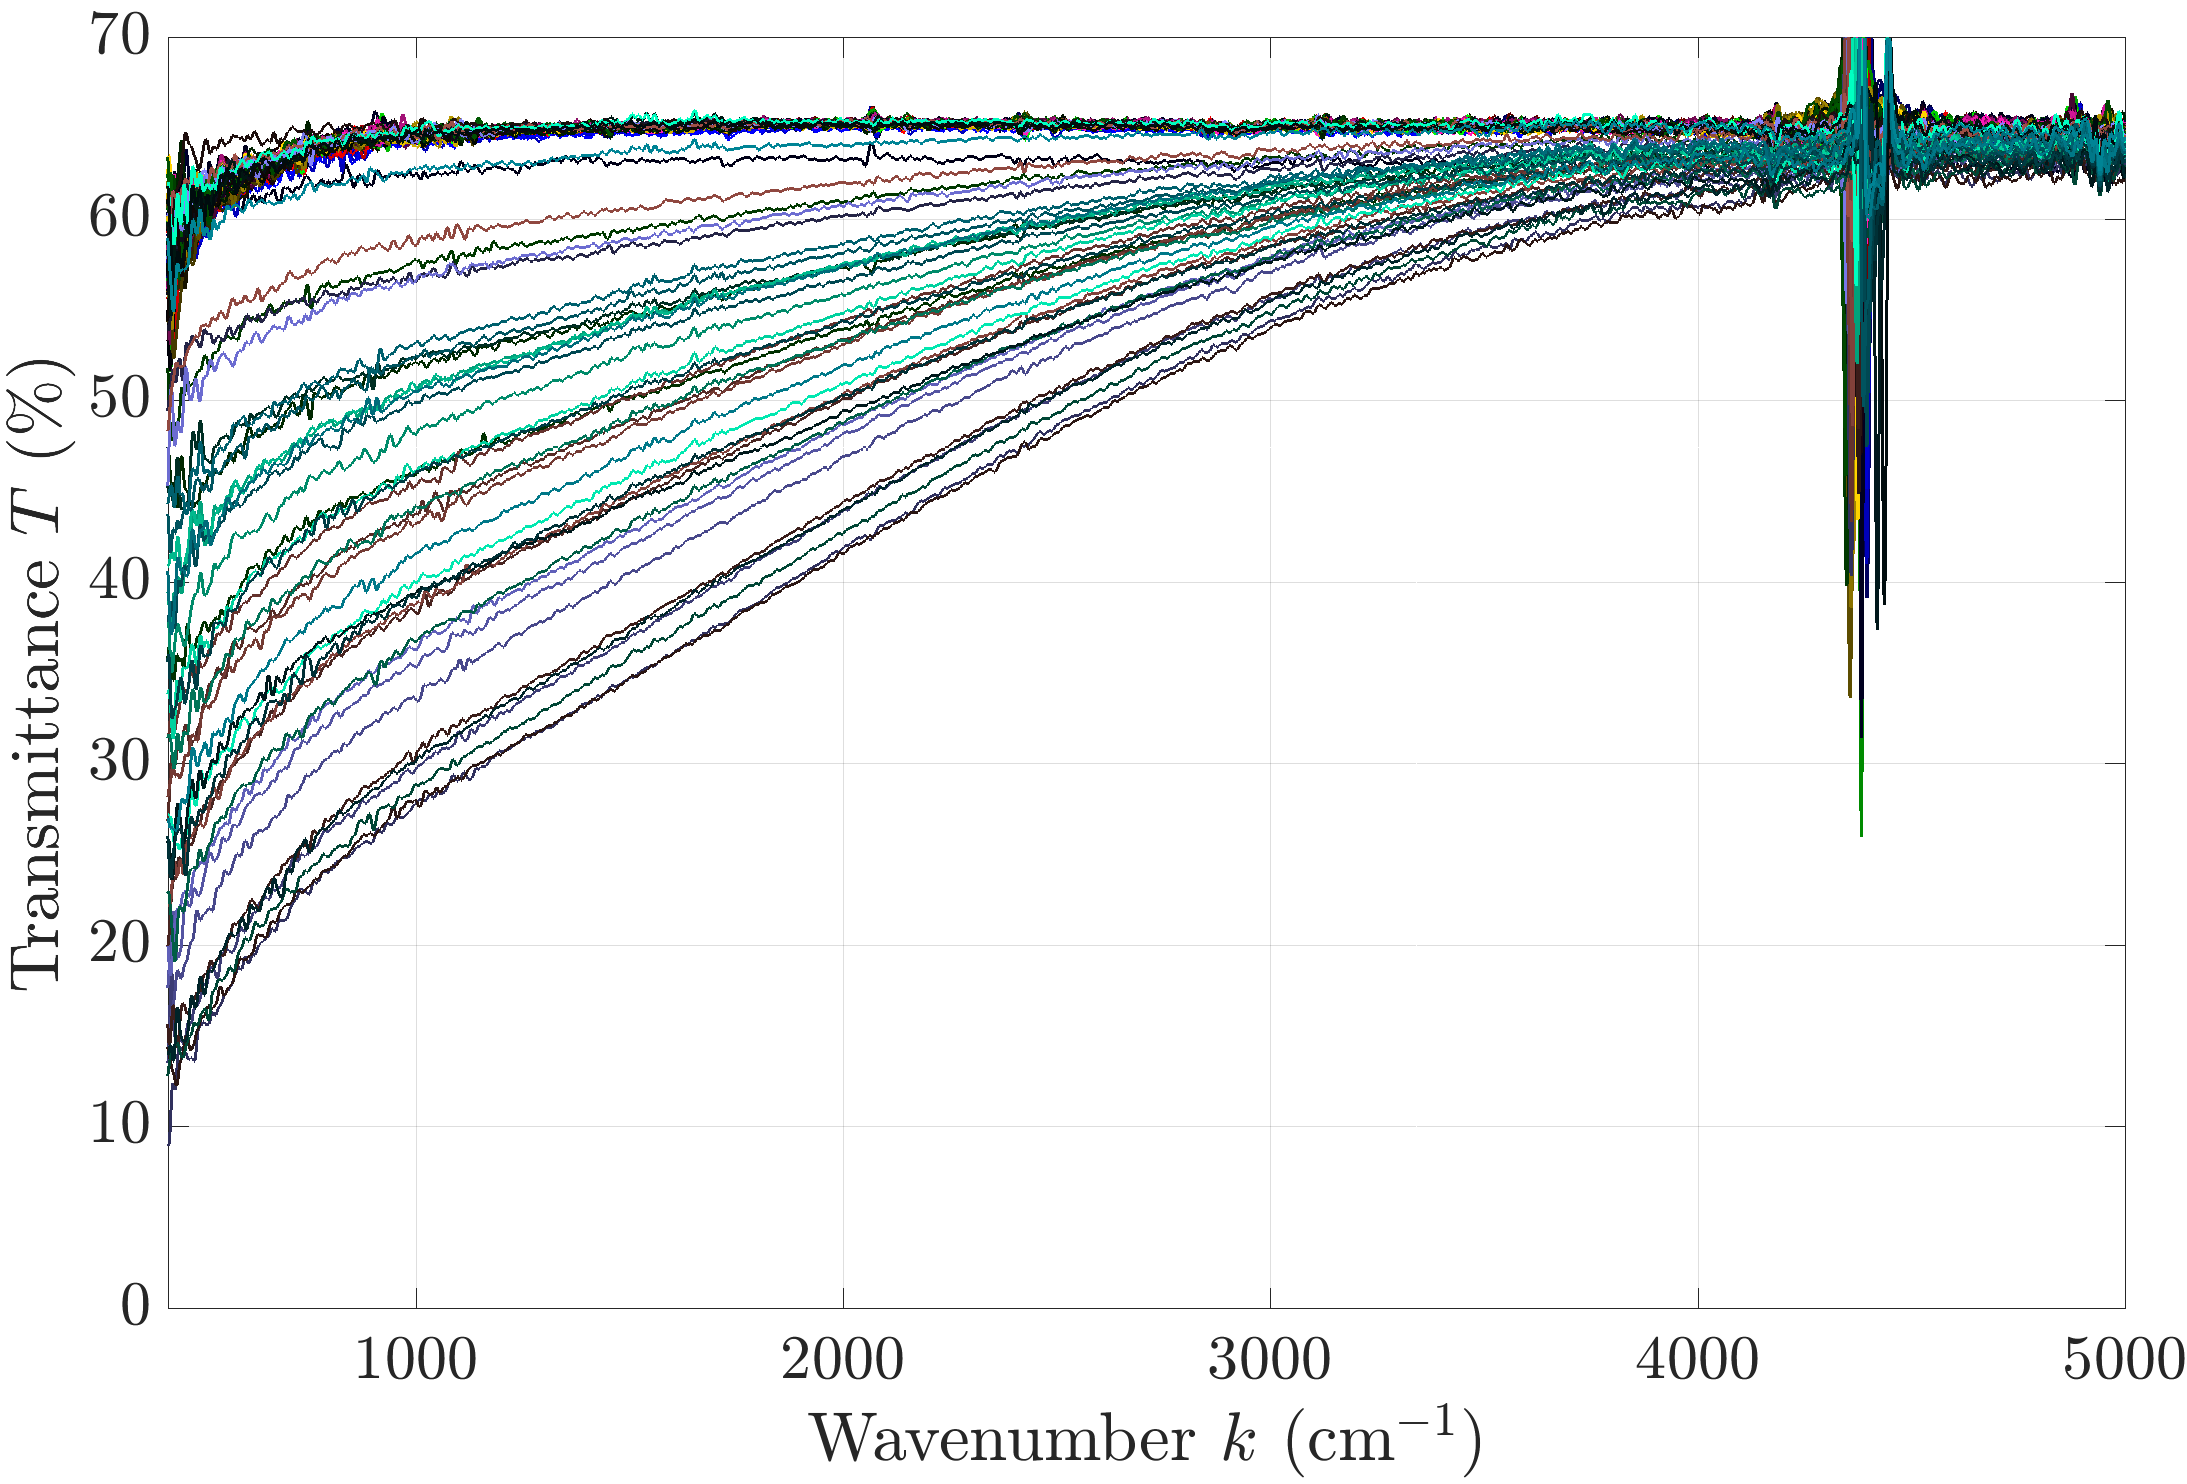
\includegraphics[width=\linewidth]{subB2a_121_ftir_spectra.png}
        \caption{}\label{fig:subB2a_ftir_spectra}
    \end{subfigure}
    \hfill
    \begin{subfigure}[t]{0.37824561403\linewidth}
        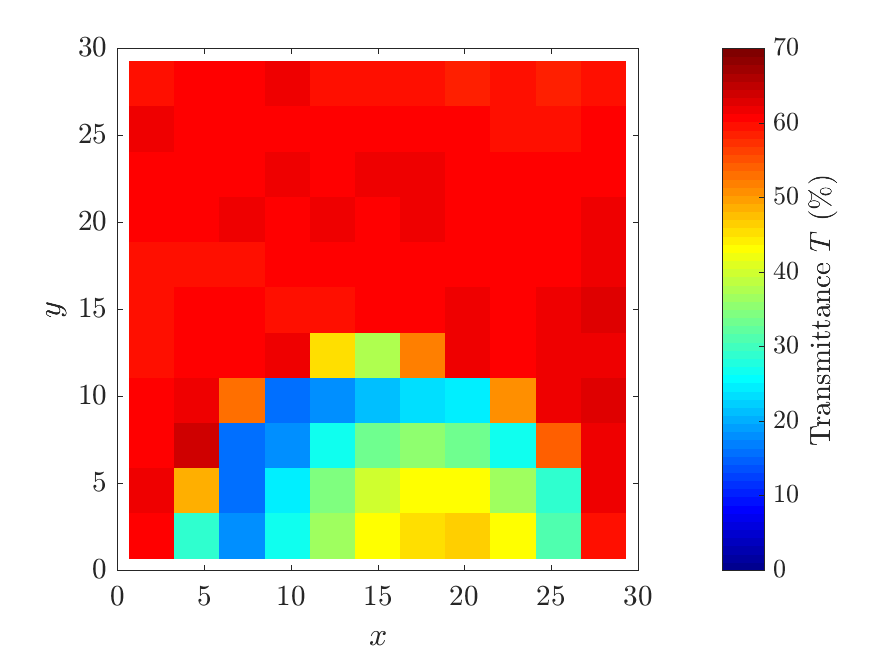
\includegraphics[width=\linewidth]{subB2a_121_ftir_transmission_at_k500cm-1.png}
        \caption{}\label{fig:subB2a_ftir_map_500cm-1}
    \end{subfigure}
    \caption[\Ac{ftir} measurements of the as-received substrate B2.]{\Acf{ftir} measurements recorded from a $11\times11$ grid on the as-received (111)B-oriented substrate B2: \subref{fig:subB2a_ftir_spectra} Transmission spectra; \subref{fig:subB2a_ftir_map_500cm-1} transmission map at wavenumber $k=\SI{500}{\centi\metre^{-1}}$ showing the transmittance $T$ in percentage of incoming light that is transmitted through at each grid point.}
\end{figure}

\todo{Beskriv} Fig.~\ref{fig:subB2a_ftir_map_500cm-1}. 

The area of lower transmission form a semicircle in the lower part of substrate B2. Surprisingly, this semicircle is visible as a brighter area in \ac{sem}, see Fig.~\ref{fig:subB2b_sem_low_transmission}. It begins \SI{4.11}{\milli\metre} from the left edge, goes around up to about \SI{13.11}{\milli\metre} before it goes down, and ends \SI{1.89}{\milli\metre} from the right edge. The major influence on \ac{se} generation is the topography of the surface. Generally, edges and other pointy parts that are produce more \acp{se}, and hence, these parts look brighter than the rest of the image \citep{goldstein2012scanning}. This is not the case for the brighter area since the surface is as uniform and smooth as the surrounding substrate. Also, the average atomic number influence the contrast, but \ac{eds} spectra confirms that the low transmission area and the surrounding substrate have the same composition.

It could be different crystal orientation that cause the contrast in the \ac{sem} images in Fig.~\ref{fig:subB2b_sem_low_transmission}, like for the twins on substrate B. 

\begin{figure}
    \centering
    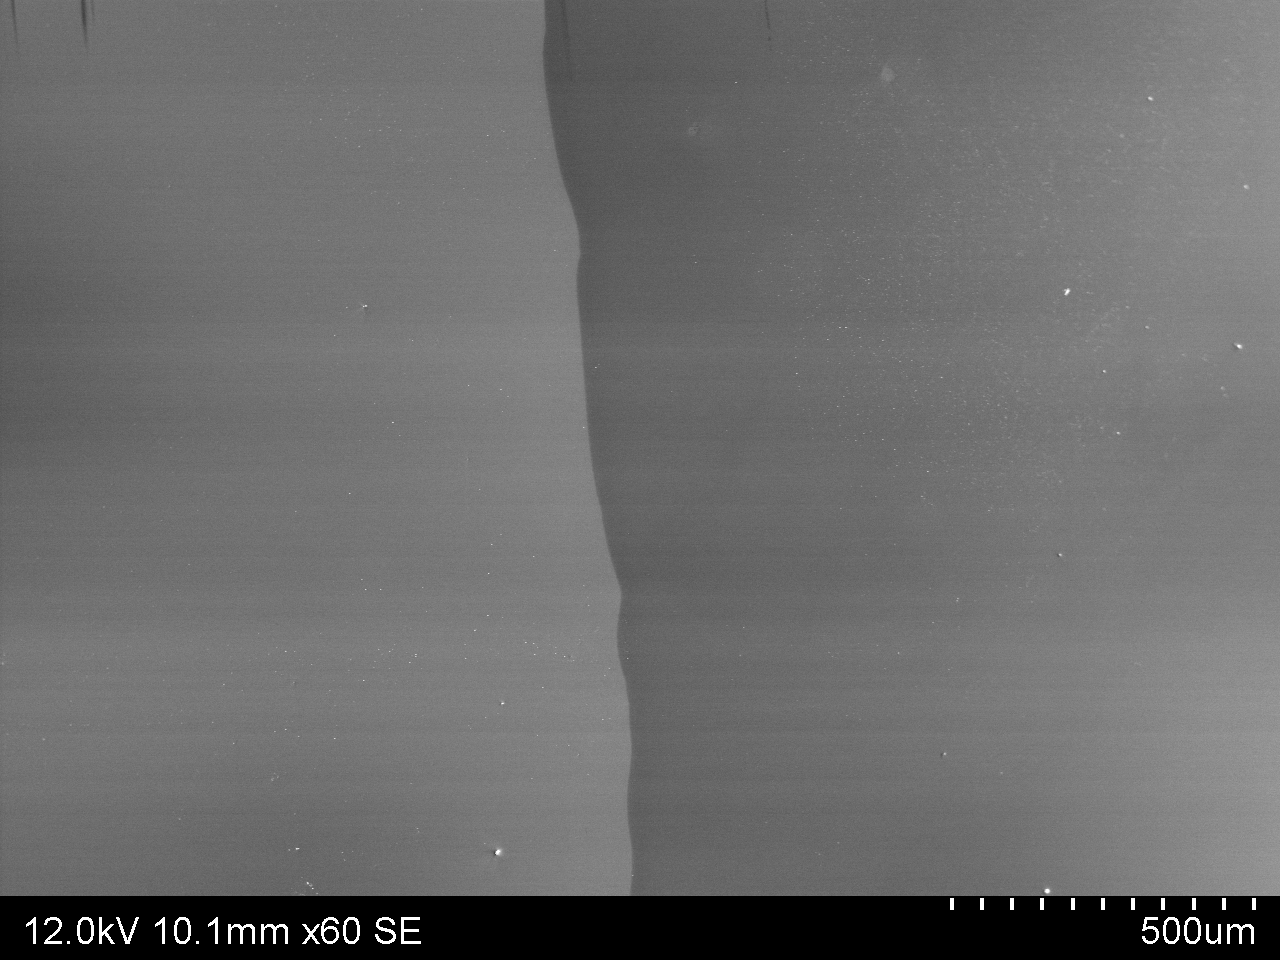
\includegraphics[width=1.0\linewidth]{subB2b_sem_04_m005.png}
    %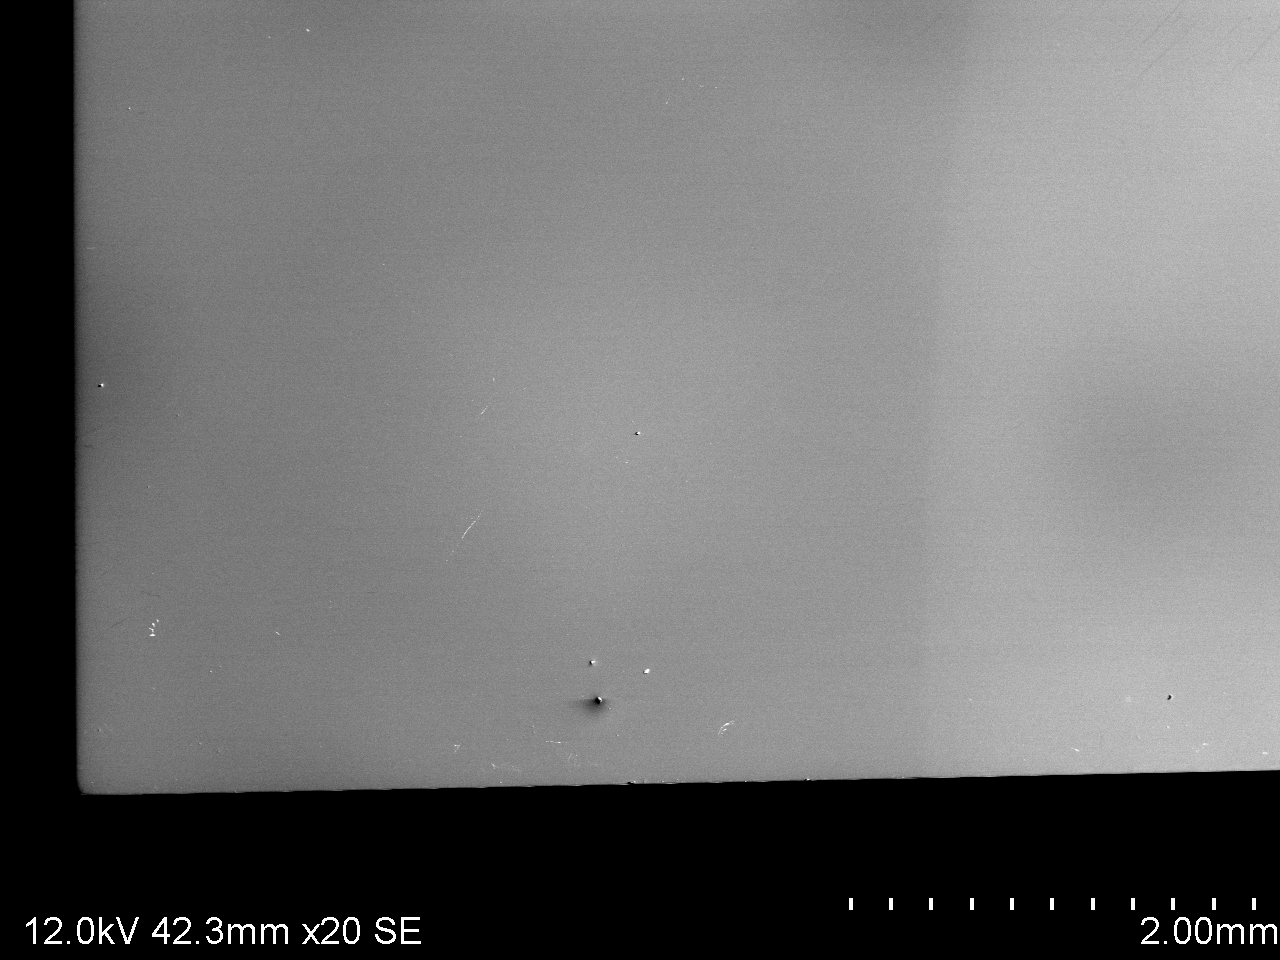
\includegraphics[width=1.0\linewidth]{subB2b_sem_05_m002.png}\caption{Left edge}
    %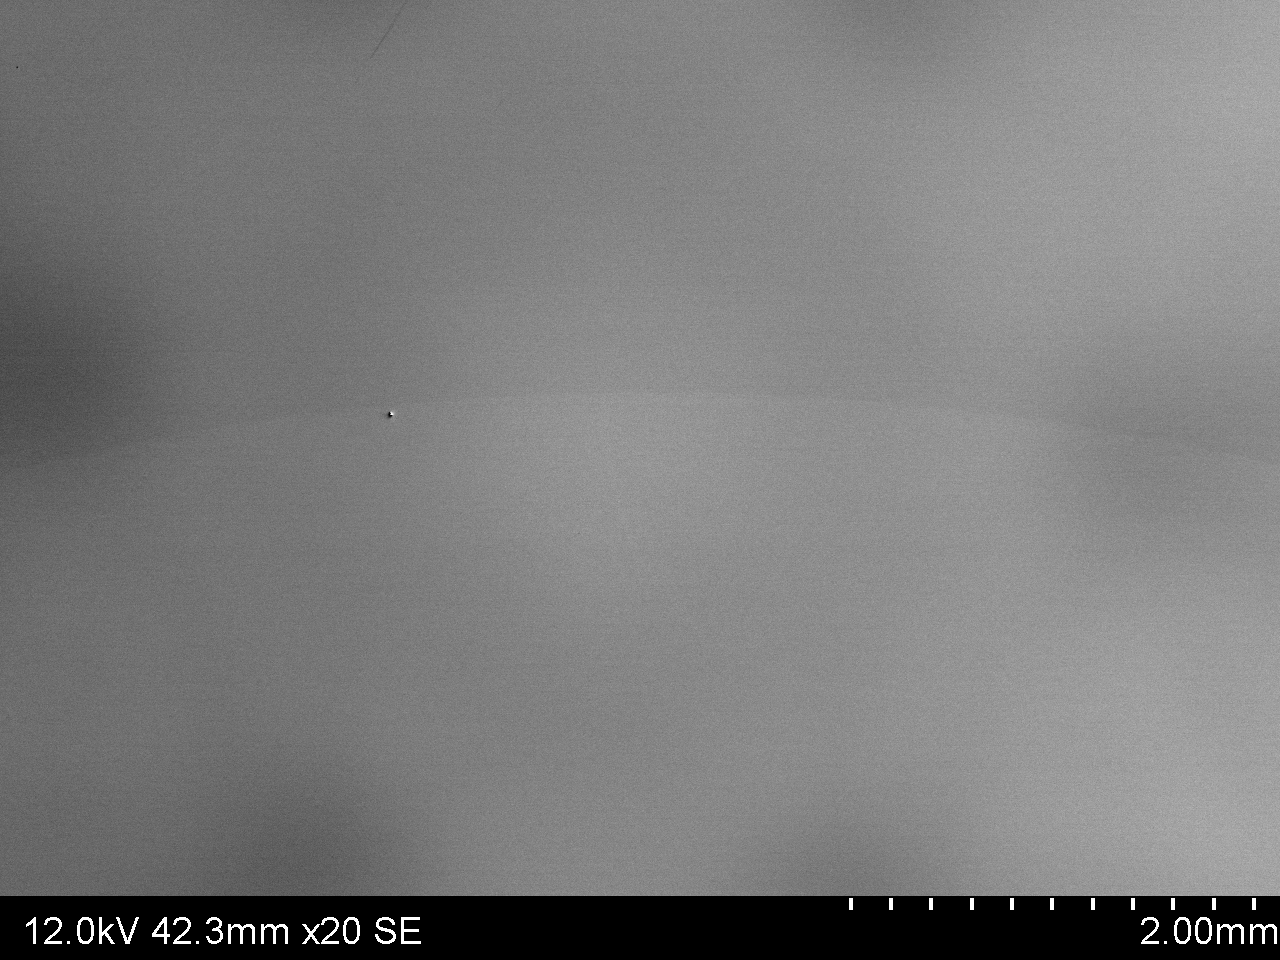
\includegraphics[width=1.0\linewidth]{subB2b_sem_05_m005.png}\caption{Upper edge}
    %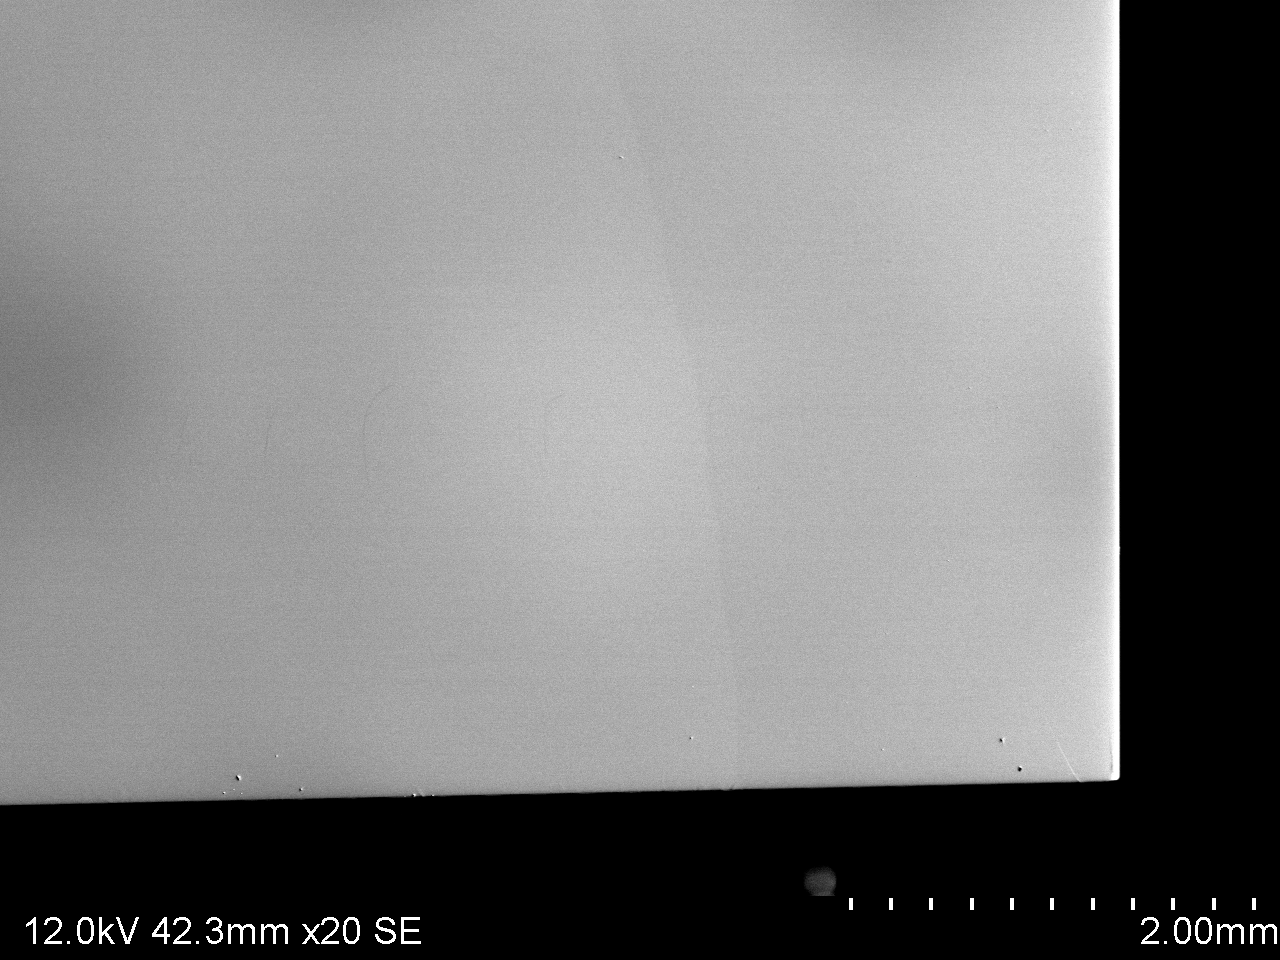
\includegraphics[width=1.0\linewidth]{subB2b_sem_05_m003.png}\caption{Right edge}
    \caption[]{\Ac{sem} image of the right edge of the semicircle with low \ac{ir} transmission in the lower part of substrate B2. The semicircle appears brighter than the rest of the substrate surface.}\label{fig:subB2b_sem_low_transmission}
\end{figure}

%%========================================
